%!TeX encoding = UTF-8 Unicode
\documentclass{article}
\usepackage[pdftex]{graphicx} %for embedding images
\usepackage{url} %for proper url entries
\usepackage[bookmarks, colorlinks=false, pdfborder={0 0 0}, pdftitle={Laboratory ML Project 01}, pdfauthor={Nhut-Nam Le}, pdfsubject={Introduction to Machine Learning}, pdfkeywords={report, exercises}]{hyperref} %for creating links in the pdf version and other additional pdf attributes, no effect on the printed document
%\usepackage[final]{pdfpages} %for embedding another pdf, remove if not required
\usepackage[utf8]{inputenc}
\usepackage[english, vietnamese]{babel}
\usepackage{float}
\usepackage{fancyhdr}
\usepackage{pythonhighlight}
\usepackage[left=3cm, right=3cm, top=2cm, bottom=2cm]{geometry}
\usepackage{parskip}
\usepackage{tikz}
\usepackage{hyperref}
\usepackage[]{algorithm2e}
\usepackage[noend]{algpseudocode}
\usepackage{amsmath}
\usepackage{amsfonts}

\usepackage{listings}
\usepackage{color}

\definecolor{dkgreen}{rgb}{0,0.6,0}
\definecolor{gray}{rgb}{0.5,0.5,0.5}
\definecolor{mauve}{rgb}{0.58,0,0.82}

\newcommand\T{\rule{0pt}{2.6ex}}       % Top strut
\newcommand\B{\rule[-1.2ex]{0pt}{0pt}} % Bottom strut


\lstset{frame=tb,
	language=Java,
	aboveskip=3mm,
	belowskip=3mm,
	showstringspaces=false,
	columns=flexible,
	basicstyle={\small\ttfamily},
	numbers=none,
	numberstyle=\tiny\color{gray},
	keywordstyle=\color{blue},
	commentstyle=\color{dkgreen},
	stringstyle=\color{mauve},
	breaklines=true,
	breakatwhitespace=true,
	tabsize=3
}

\setlength{\parindent}{15pt}
\setlength{\headheight}{15.2pt}
\pagestyle{fancy}
\lhead[<even output>]{NHẬP MÔN HỌC MÁY}
\rhead[<even output>]{BÁO CÁO ĐỒ ÁN THỰC HÀNH 01}
\title{research-outline}
\author{Nhut-Nam Le}
\date{2021}
\begin{document}
	\begin{titlepage}
		\begin{center}
			% Top of the page
			\large{\textbf{ĐẠI HỌC KHOA HỌC TỰ NHIÊN, ĐHQG-HCM\\KHOA CÔNG NGHỆ THÔNG TIN\\BỘ MÔN KHOA HỌC MÁY TÍNH}}\\
			
\includegraphics[width=0.75\textwidth]{images/khtn.png}\\
			% Title
			\large \textbf{NHẬP MÔN HỌC MÁY}\\[0.1in]
			\huge \textbf{BÁO CÁO ĐỒ ÁN THỰC HÀNH}\\[0.1in]
			\huge \textbf{REGRESSION - HỒI QUY}\\[0.1in]
			\vfill
			\normalsize
			% Submitted by
			\normalsize
			% Lecturers
			\textbf{Giảng viên lý thuyết}\\
			{\textbf{TS.} Bùi Tiến Lên}\\[0.1in]
			% Teacher Assistant
			\textbf{Giảng viên hướng dẫn}\\
			\vspace{0.1in}
			{Dương Nguyễn Thái Bảo, Nguyễn Ngọc Đức, Nguyễn Tiến Huy, Lê Thanh Phong}\\[0.1in]
			\textbf{Sinh viên thực hiện} \\
			\vspace{0.1in}
			% Submitted by
			{Vương Gia Bảo, Ngô Xuân Kiên, Lê Nhựt Nam, Nguyễn Viết Dũng}\\[0.1in]
			% Date time when written report
			\vfill
			Tháng 5 năm 2021
		\end{center}
	\end{titlepage}
	\newpage
	% End Title4
	
	\pagenumbering{roman} %numbering before main content starts
	\cleardoublepage
	%\pagebreak
	\phantomsection
	\addcontentsline{toc}{section}{Lời cảm ơn}
	\section*{Lời cảm ơn}
	\vspace{1.0in}
	\begingroup
	\setlength{\parindent}{0pt}
	\qquad Trong quá trình thực hiện đồ án này, chúng em đã nhận được rất nhiều sự giúp đỡ cũng như hỗ trợ từ các thầy cô Trường Đại học Khoa học Tự nhiên, ĐHQG-HCM và các bạn bè trong lớp Nhập môn Học Máy. Chúng em xin bày tỏ lòng cảm ơn chân thành đến mọi người vì đã giúp đỡ hướng dẫn, chỉ bảo rất tận tình.
	
	\qquad Đặc biệt, chúng em xin bày tỏ lòng biết ơn sâu sắc đến các thầy cô khoa Công nghệ Thông tin, cụ thể hơn là thầy Bùi Tiến Lên và các thầy hướng dẫn đã giảng dạy rất nhiệt, cung cấp nhiều slides, tài nguyên học tập cần thiết, tạo điều kiện tốt nhất để chúng em có thể hoàn thành được đồ án này.
	
	\qquad Trong quá trình, viết báo cáo này, chúng em không thể tránh khỏi nhiều thiếu sót, hy vọng mong nhận được góp ý từ thầy để chúng em tiếp tục hoàn thiện hơn đối với đồ án này, cũng như rút kinh nghiệm cho những đồ án, những báo cáo kế tiếp.
	
	\vspace{1.0in}
	\textbf{Đại học Khoa học Tự nhiên, ĐHQG-HCM.}\\
	Vương Gia Bảo, Ngô Xuân Kiên, Lê Nhựt Nam, Nguyễn Viết Dũng\\
	Tháng 4 năm 2021\\
	\endgroup
	
	\newpage
	\tableofcontents
	\newpage
	\pagenumbering{arabic} %reset numbering to normal for the main content
	\setcounter{secnumdepth}{0}
	
	\section{Thông tin nhóm}
	\begin{table}[H]
		\centering
		\begin{tabular}{ | p{1cm} |  p{3cm} | p{5cm} | p{5cm}  |}\hline
			STT	& MSSV & Họ tên đầy đủ & Email liên lạc \\\hline
			1 & 18120009 & Vương Gia Bảo & 18120009@student.hcmus.edu.vn  \\ \hline
			2 & 18120045 & Ngô Xuân Kiên & 18120045@student.hcmus.edu.vn \\ \hline
			3 & 18120061 & Lê Nhựt Nam & 18120061@student.hcmus.edu.vn  \\ \hline
			4 & 18120167 & Nguyễn Viết Dũng &  18120167@student.hcmus.edu.vn \\ \hline
		\end{tabular}
	\end{table}
	\section{Phân công công việc}
	\begin{table}[H]
		\begin{tabular}{ | l | l | l | p{5.5cm} | p{3cm} |}
			\hline
			STT & MSSV & Họ tên & Nội dung công việc & Mức độ hoàn thành  \\ \hline
			1 & 18120009 & Vương Gia Bảo & Thu thập dữ liệu, đọc hiểu source, báo cáo Introduction Paper &  100\%\T\B\\ \hline
			2 & 18120045 & Ngô Xuân Kiên & Thu thập dữ liệu, đọc hiểu source, báo cáo Related Work Paper & 100\%\T\B \\ \hline
			3 & 18120061 & Lê Nhựt Nam & Thu thập dữ liệu, đọc hiểu source, báo cáo, SincNet Architecture, Slides thuyết trình, Midterm Report & 100\%\T\B \\ \hline
			4 & 18120167 & Nguyễn Viết Dũng &  Thu thập dữ liệu, đọc hiểu source, báo cáo experimental setup Paper & 100\%\T\B \\ \hline
		\end{tabular}
	\end{table}
	\section{Tiêu chí đánh giá đồ án}
	\subsection{Bảng tiêu chí cho đồ án}
	\begin{table}[H]
		\begin{tabular}{ | p{5cm} | p{6.5cm} | p{3cm} |}\hline
			Tên tiêu chí đồ án & Nội dung tiêu chí & Mức độ hoàn thiện  \T\B\\\hline
			Nhận diện bài toán & Sinh viên cần tìm hiểu bài toán và dữ liệu được giao
			nhằm xác định nội dung và ý nghĩa bài toán thực tế cần giải quyết. Thông
			qua đó, sinh viên có khả năng ánh xạ vấn đề thực tế sang bài toán lập trình & 100\%  \T\B\\\hline
			Giải quyết vấn đề & Sinh viên được yêu cầu đưa ra các giải pháp và hướng
			tiếp cận nhằm giải quyết được yêu cầu bài toán thực tế & 100\%  \T\B\\\hline
			Xử lý và phân tích dữ liệu & Sinh viên có khả năng xử lý các công cụ phân
			tích dữ liệu tự động nhằm tìm ra các thông tin hữu ích, các đặc trưng tiềm ẩn
			ảnh hưởng để mục tiêu bài toán &100\%  \T\B\\\hline
			Thiết kế và cài đặt các thuật toán máy học & Sinh viên được yêu cầu có
			khả năng đề xuất, triển khai và giải thích các thuật toán máy học nhằm giải
			quyết bài toán được giao & 100\%  \T\B\\\hline
		\end{tabular}
	\end{table}
	\subsection{Bảng yêu cầu cho đồ án}
	\begin{table}[H]
		\begin{tabular}{ | p{5cm} | p{6.5cm} | p{3cm} |}\hline	
			Tên yêu cầu & Nội dung yêu cầu & Mức độ hoàn thiện  \T\B\\\hline
			Phân tích dữ liệu & Đọc và phân tích các đặc trưng trong 2 tập tin được cung cấp. Trình bày các thông tin hữu ích (insights) tác động đến chi phí y tế cá nhân & 100\%  \T\B\\\hline
			Cài đặt thuật toán & Cài đặt các thuật toán máy học đã được học để dự đoán chi phí y tế cá nhân. & 100\%  \T\B\\\hline
			Trình bày kết quả và nhận xét & Báo cáo kết quả đạt được sau quá trình phân tích và cài đặt. Từ đó nhận xét về các tác nhân ảnh hưởng mạnh/yếu tới chi phí y tế cá nhân & 100\%  \T\B\\\hline
		\end{tabular}
	\end{table}	
	\subsection{Bảng danh sách các thuật toán Hồi quy}
	\begin{table}[H]
		\begin{tabular}{ | p{3cm} | p{5cm} | p{3cm} | p{3cm} |} \hline	
			Thuật toán máy học & Cách cài đặt & Thư viện để đối chiếu (Nếu có) & Đánh giá hoàn thành\T\B\\\hline
			Multi Linear Regression & & & 100\%  \T\B\\\hline
			Logistic Regression & & & 100\%  \T\B\\\hline
			Ridge Regression & & & 100\%  \T\B\\\hline
			Lasso Regression & & & 100\%  \T\B\\\hline
			Random Forest Regressor & & & 100\%  \T\B\\\hline
			Polynomial Regression & & & 100\%  \T\B\\\hline
		\end{tabular}
	\end{table}		
	\section{Nội dung báo cáo}
	
	\section{1. Đọc dữ liệu}
	\qquad Để cho thuận tiện trong quá trình demo trên môi trường \textbf{Google Colab} nhóm chúng em sử dụng lệnh wget trên Linux, dowload trực tiếp dữ liệu từ đường dẫn mà thầy đã public trong bài lab này.
	\begin{figure}[H]
		\centering
		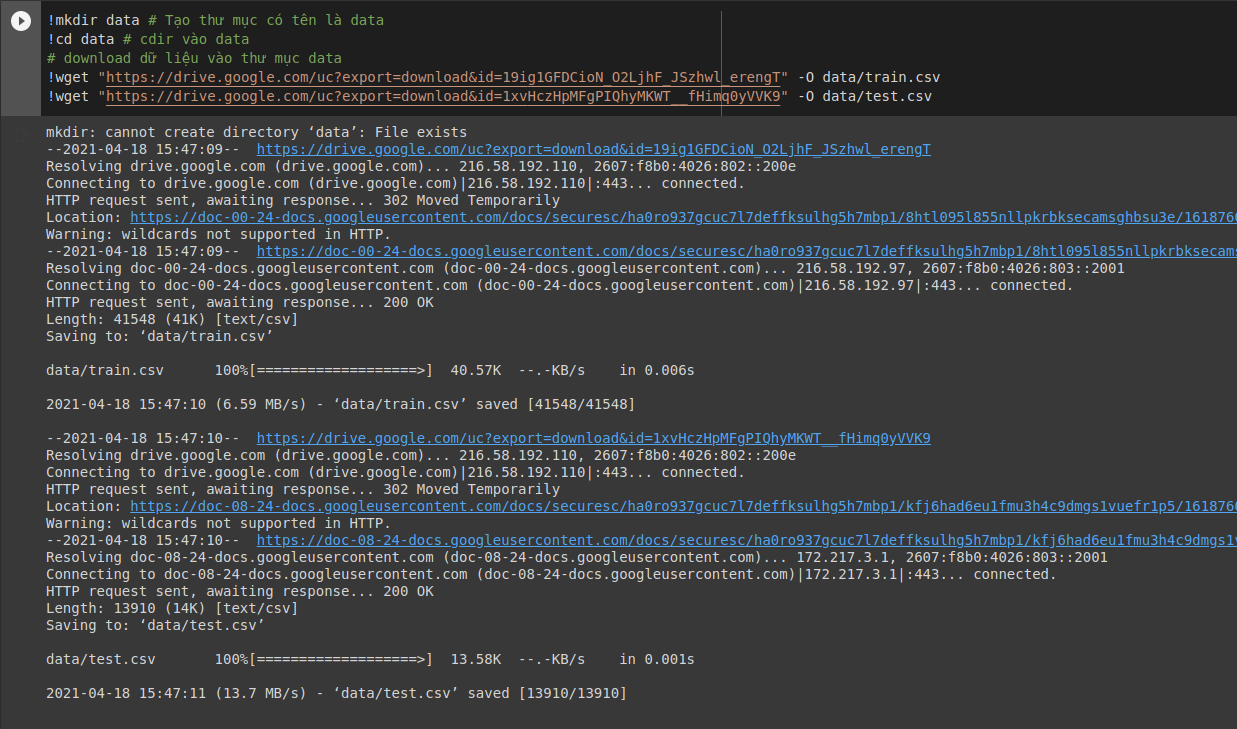
\includegraphics[width=1\textwidth]{images/download_data.png}
		\caption{Download dữ liệu: train data, test data}
		\label{fig:writing-thesis-dowload-data}
	\end{figure}
	
	Phần import một số thư viện cần thiết cho việc nhập xuất dữ liệu, xử lý dữ liệu dạng bảng, trực quan hóa dữ liệu, thư viện cung cấp các mô hình máy học
	\begin{figure}[H]
		\centering
		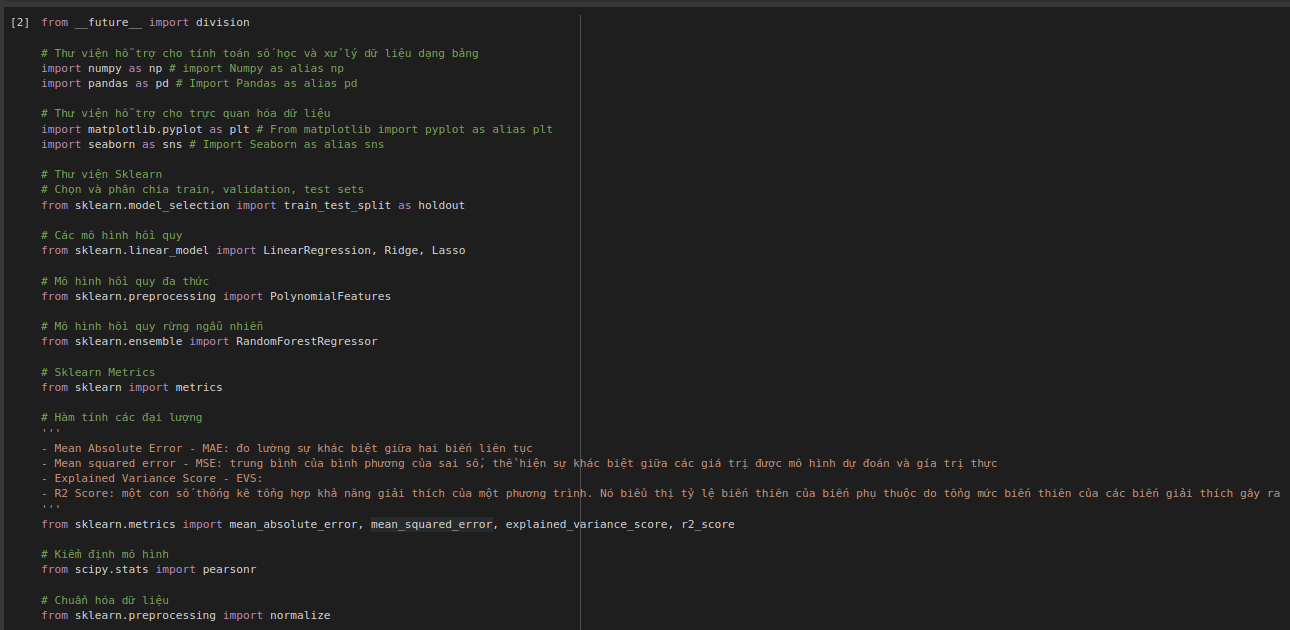
\includegraphics[width=1\textwidth]{images/import_section.png}
		\caption{Import các thư viện hỗ trợ}
		\label{fig:writing-thesis-import-section}
	\end{figure}
	
	Phần đọc dữ liệu, sử dụng thư viện Pandas như sau
	\begin{figure}[H]
		\centering
		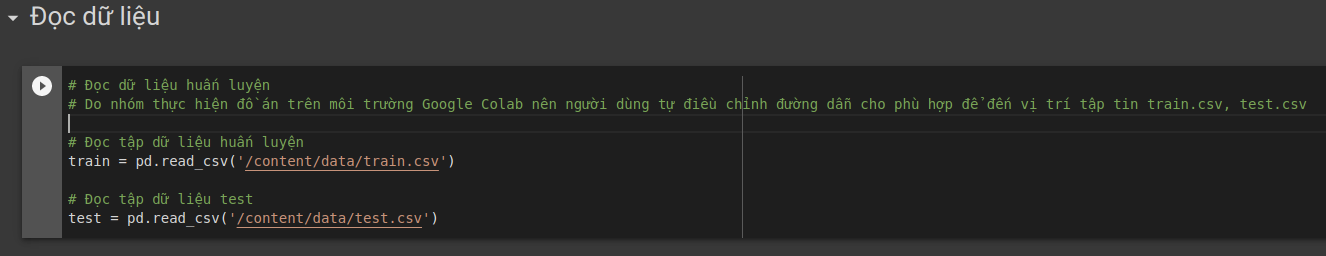
\includegraphics[width=1\textwidth]{images/read_train_test.png}
		\caption{Đọc dữ liệu}
		\label{fig:writing-thesis-read-train-test-data}
	\end{figure}
	
	\section{2. Phân tích dữ liệu}
	
	\subsection{1. Tổng quan dữ liệu thông qua các đại lượng thống kê cơ bản}
	\begin{figure}[H]
		\centering
		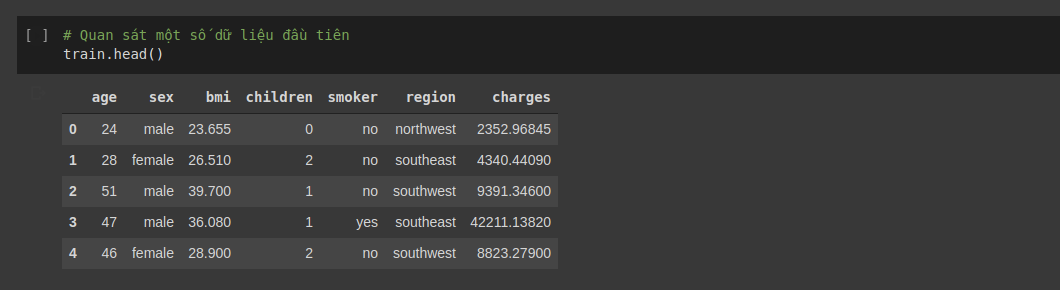
\includegraphics[width=1\textwidth]{images/train_head.png}
		\caption{Hiển thị một phần dữ liệu huấn luyện đầu tiên}
		\label{fig:writing-thesis-train-head}
	\end{figure}
	
	\subsection{2. Các đại lượng thống kê cơ bản của đặc trưng chi phí y tế}
	\begin{figure}[H]
		\centering
		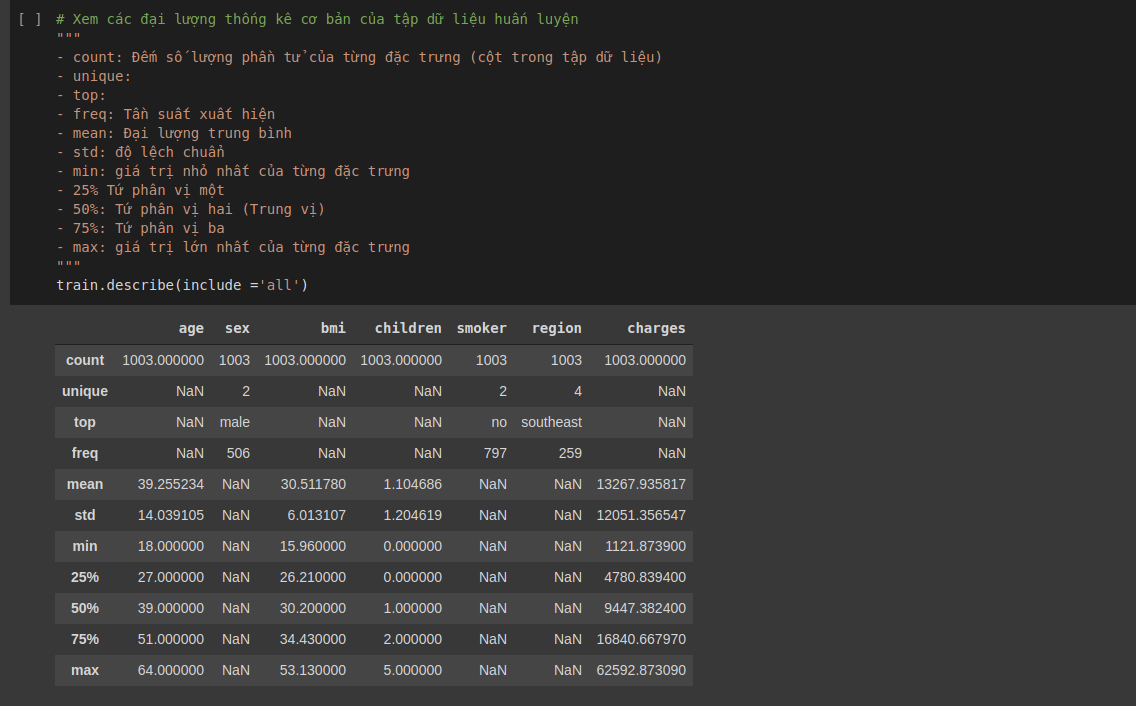
\includegraphics[width=1\textwidth]{images/simple_stat_on_train_set.png}
		\caption{Thống kê mô tả trên tập huấn luyện}
		\label{fig:writing-thesis-simple-stat-on-train-set}
	\end{figure}

	\begin{figure}[H]
		\centering
		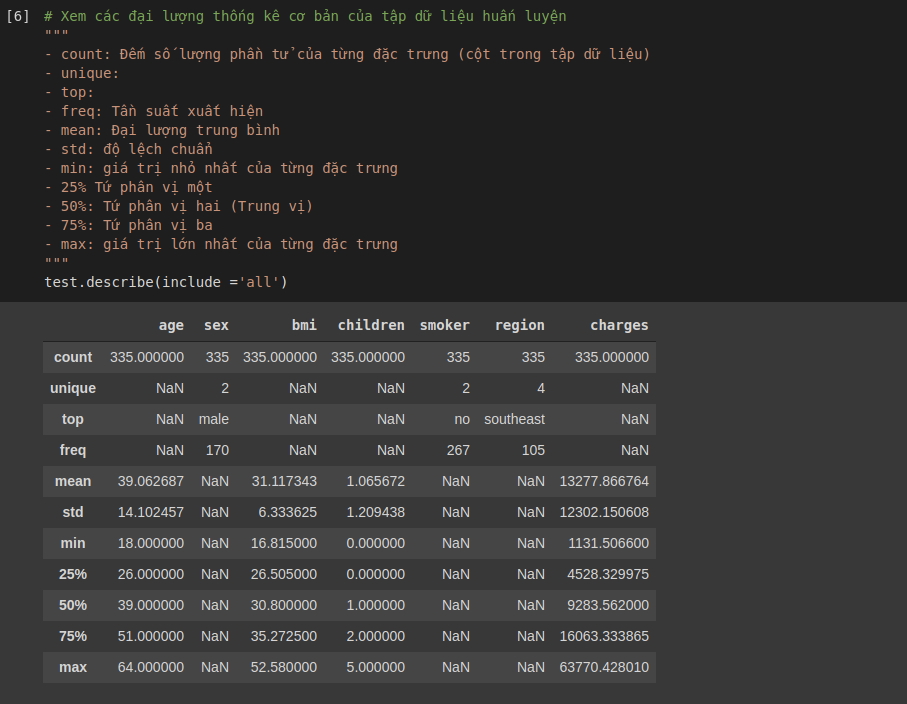
\includegraphics[width=1\textwidth]{images/simple_stat_on_test_set.png}
		\caption{Thống kê mô tả trên tập kiểm tra}
		\label{fig:writing-thesis-simple-stat-on-test-set}
	\end{figure}

	\begin{figure}[H]
		\centering
		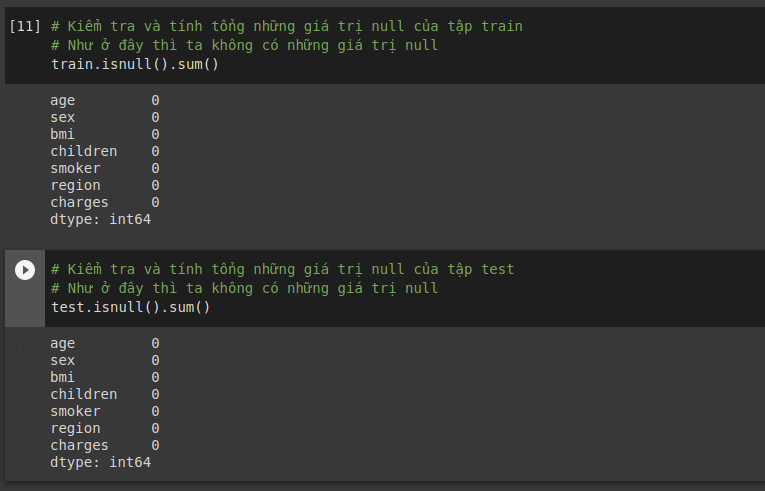
\includegraphics[width=1\textwidth]{images/check_null_train_test.png}
		\caption{Kiểm tra null values trên hai tập: tập huấn luyện, tập kiểm tra}
		\label{fig:writing-thesis-check-null-train-test}
	\end{figure}

	\begin{figure}[H]
		\centering
		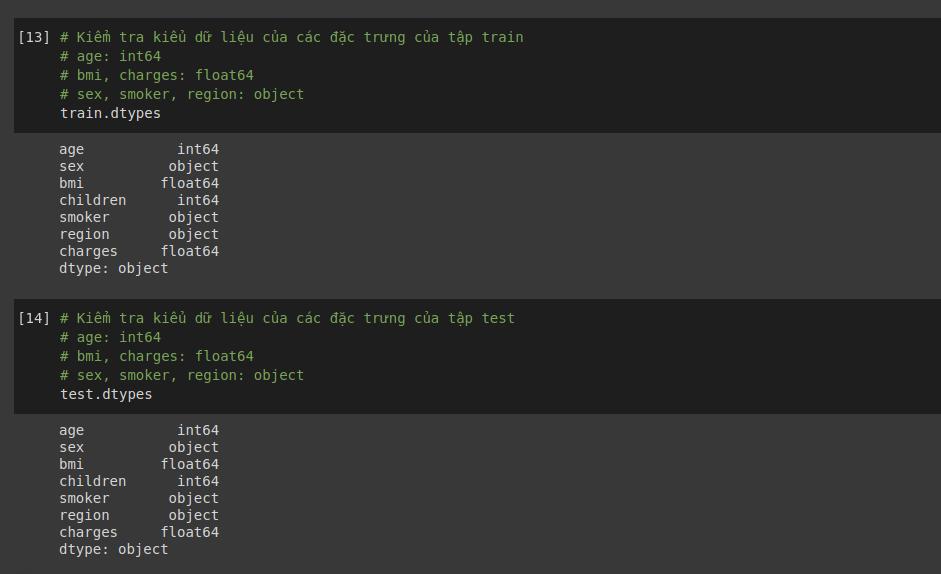
\includegraphics[width=1\textwidth]{images/data_types_train_test.png}
		\caption{Kiểm tra kiểu dữ liệu trên hai tập: tập huấn luyện, tập kiểm tra}
		\label{fig:writing-thesis-data-type-train-test}
	\end{figure}

	
	\subsection{3. Mối tương quan giữa các đặc trưng trong dữ liệu}
	\begin{figure}[H]
		\centering
		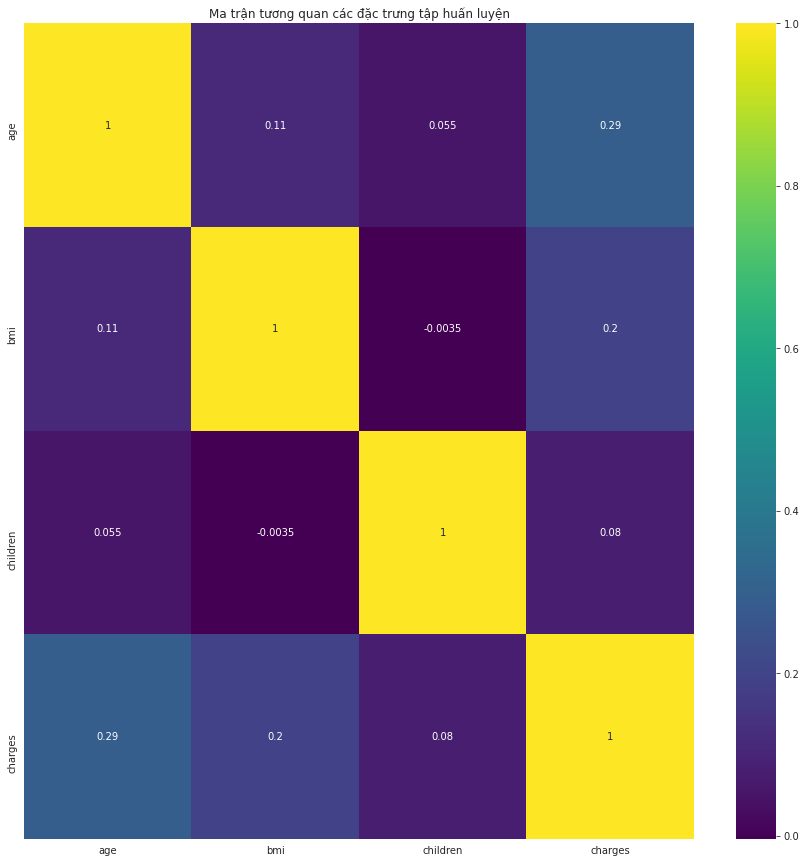
\includegraphics[width=0.7\textwidth]{images/corr_matrix_train.png}
		\caption{Ma trận tương quan giữa các đặc trưng trong tập huấn luyện}
		\label{fig:writing-thesis-corr-matrix-train}
	\end{figure}
	
	\begin{figure}[H]
		\centering
		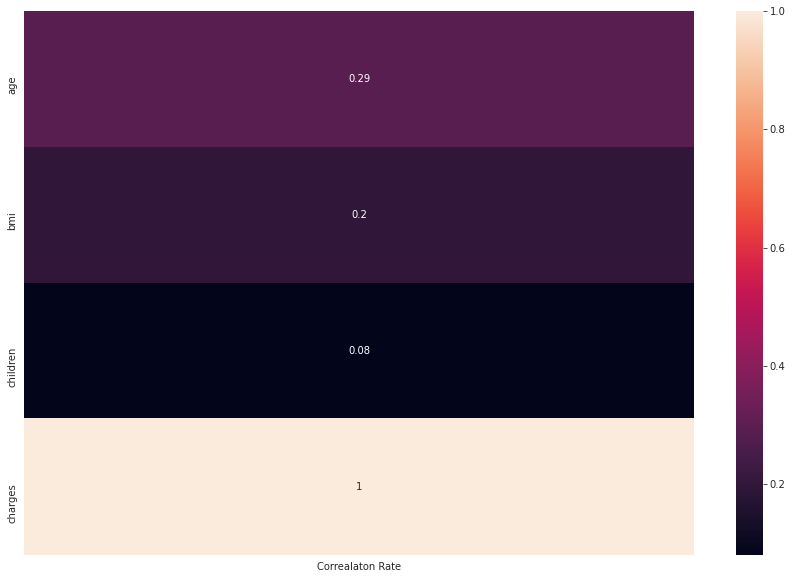
\includegraphics[width=0.7\textwidth]{images/corr_charges_other_features.png}
		\caption{Ma trận tương quan giữa chi phi y tế với các đặc trưng trong tập huấn luyện}
		\label{fig:writing-thesis-corr-charges-other-features}
	\end{figure}
	\textbf{Nhận xét:} Giữa các cặp đặc trưng dữ liệu có mối quan hệ tương đối thấp, hệ số tương quan giữa chúng bé hơn 0.5. Điều này chúng ta cần suy đoán, cần phải thêm một số điều kiện khác nữa để rút ra mối quan hệ giữa chúng với chi phí y tế: vùng (Region), tình trạng hút thuốc (Smoker) và số lượng trẻ con/ người phụ thuộc (children)
	
	\subsection{4. Phân tích đặc trưng chi phí y tế}
	\begin{figure}[H]
		\centering
		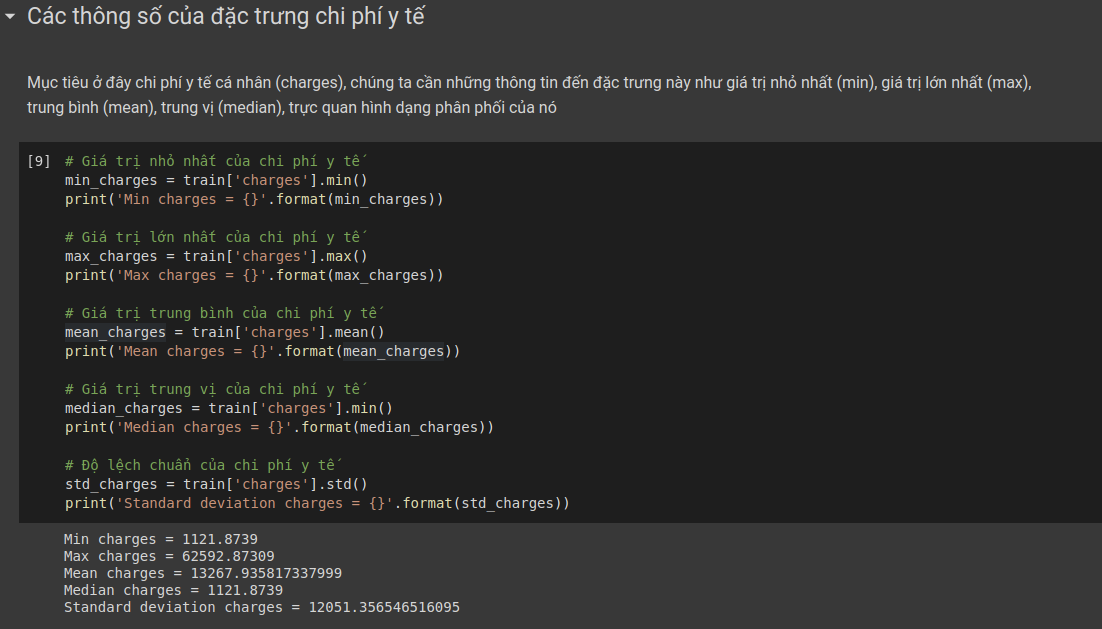
\includegraphics[width=1\textwidth]{images/medical_charges.png}
		\caption{Thông số thống kê cơ bản về đặc trưng chi phí y tế}
		\label{fig:writing-thesis-medical-charges}
	\end{figure}
	Một số thống kê cơ bản về chi phí y tế:
	\begin{itemize}
		\item  Chi phí thấp nhất của chi phí y tế - Min charges = 1121.8739
		\item  Chi phí cao nhất của chi phí y tế - Max charges = 62592.87309
		\item  Chi phí trung bình của chi phí y tế - Mean charges = 13267.935817337999
		\item  Giá trị trung vị của chi phí y tế- Median charges = 1121.8739
		\item  Độ lệch chuẩn của chi phí y tế - Standard deviation charges = 12051.356546516095
	\end{itemize}
	Trực quan phân phối của đặc trưng chi phí y tế: Dùng displot seaborn để trực quan phân phối của đặc trưng y tế
	\begin{figure}[H]
		\centering
		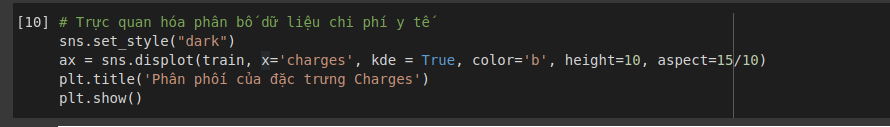
\includegraphics[width=1\textwidth]{images/dist_medical_charges.png}
		\caption{Dùng displot Seaborn để trực quan phân phối của đặc trưng chi phí y tế}
		\label{fig:writing-thesis-dist-medical-charges}
	\end{figure}
	
	\begin{figure}[H]
		\centering
		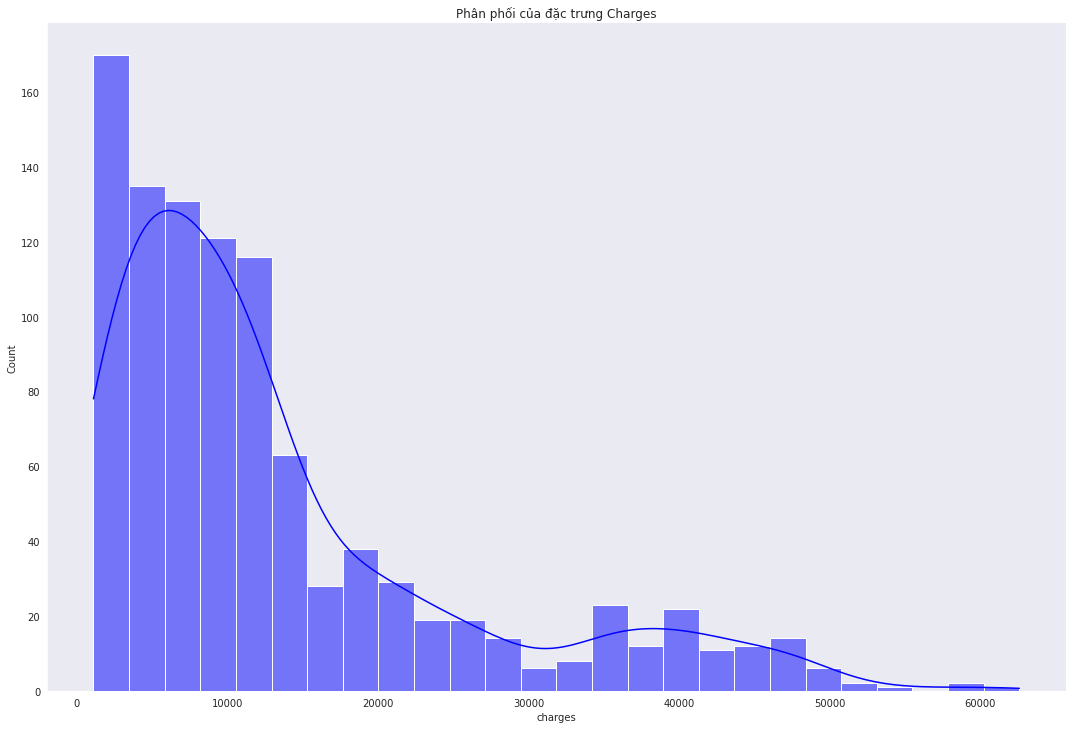
\includegraphics[width=1\textwidth]{images/dist_medical_charges_plot.png}
		\caption{Dùng displot Seaborn để trực quan phân phối của đặc trưng chi phí y tế}
		\label{fig:writing-thesis-dist-medical-charges-plot}
	\end{figure}
	\textbf{Nhận xét:} Chi phí trung bình của chi phí y tế lớn hơn rất nhiều so với Giá trị trung vị của chi phí y tế dẫn đến phân phối bị lệch sang một phía (sang trái), hình dạng phân phối này không gần phần phối chuẩn, ta có thể dùng Numpy log để tính và vẽ lại biểu dô. Hàm log và f(x) đồng biến nên sẽ không mất tính tổng quát khi xem xét phân phối của dữ liệu hay đặc trưng.

	\begin{figure}[H]
		\centering
		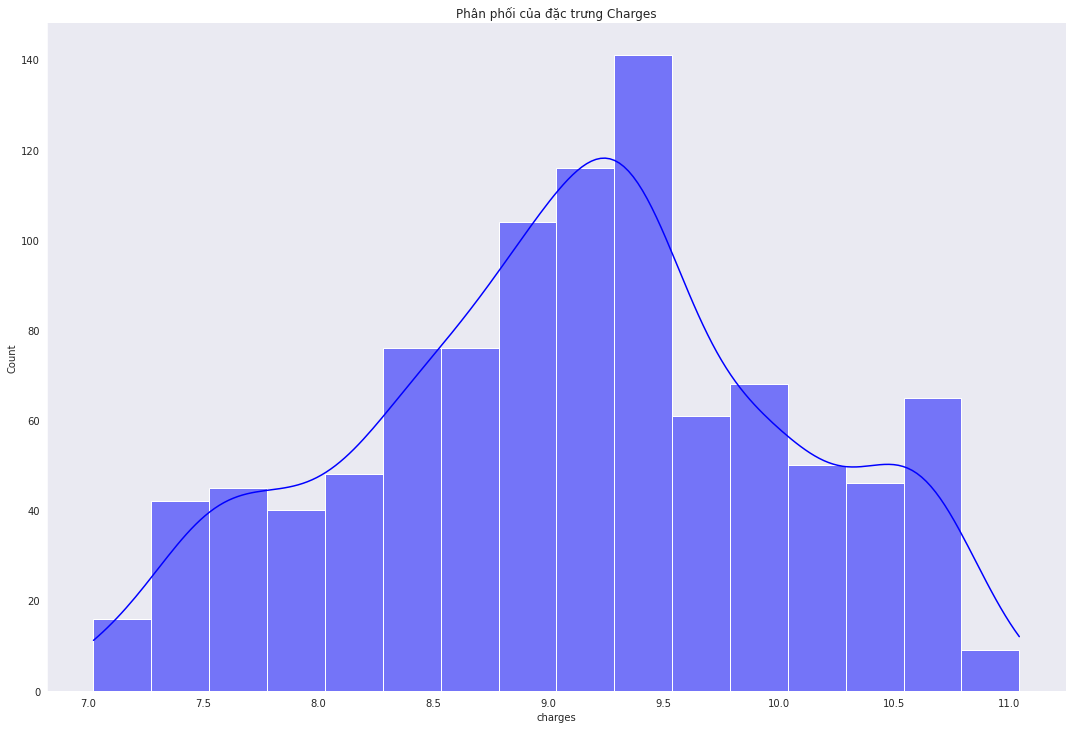
\includegraphics[width=1\textwidth]{images/dist_medical_charges_plot_log_scale.png}
		\caption{Dùng displot Seaborn để trực quan phân phối của đặc trưng chi phí y tế}
		\label{fig:writing-thesis-dist-medical-charges-plot-log-scale}
	\end{figure}
	\textbf{Nhận xét:} Hình dạng sau khi áp dụng Numpy Log, đặc trưng chi phí y tế có dạng của phân phối chuẩn, điều này cho thấy dữ liệu không có điểm bất thường.
	
	\subsection{4. Phân tích mối quan hệ chi phí y tế (charges) - vùng (region)}
	\qquad Do các giá trị trên ma trận tương quan tương đối nhỏ đối với cặp đặc trưng, nên nhóm quyết định chuyển hướng suy luận thông qua việc xem xét nhiều đặc trưng.
	
	Ở phần này, nhóm phân tích mối quan hệ giữa chi phí y tế (charges) và vùng (region)
	
	Theo như dữ liệu phía trên, đặc trưng region có 4 giá trị:
	\begin{itemize}
		\item northwest - vùng Tây Bắc
		\item northeast - vùng Đông Bắc
		\item southeast - vùng Đông Nam
		\item southwest - Vùng Tây Nam
	\end{itemize}
	Nhóm sử dụng biểu đồ cột để trực quan quá tổng giá trị chi phí ở từng vùng trên.
	\begin{figure}[H]
		\centering
		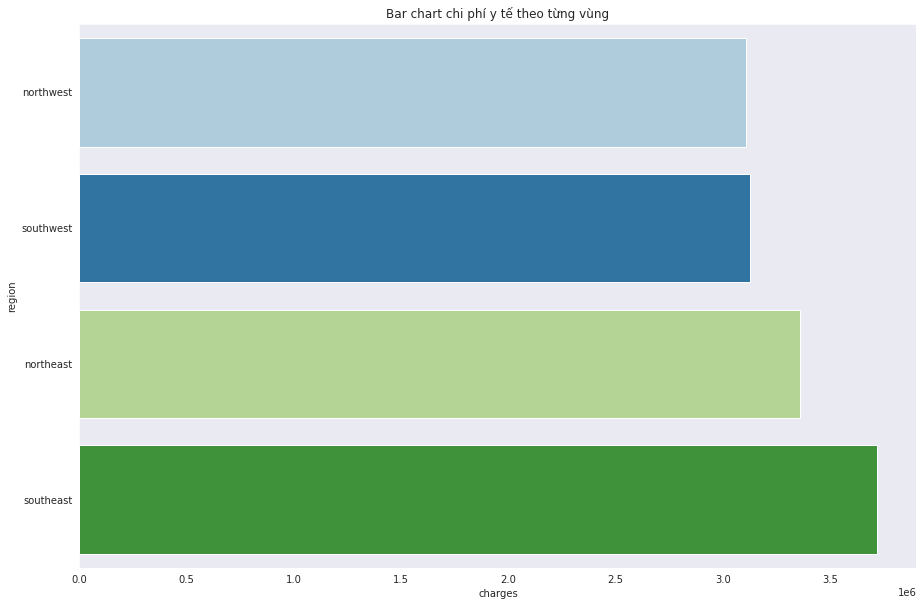
\includegraphics[width=1\textwidth]{images/bar_chart_medical_charges_region.png}
		\caption{Chi phí y tế theo từng vùng}
		\label{fig:writing-thesis-bar-chart-medical-charges-region}
	\end{figure}
	\textbf{Nhận xét:} 
	\begin{itemize}
		\item 	Biểu đồ thể hiện chi phí y tế theo từng vùng. Chúng ta có 4 vùng cần xem xét: Northwest (vùng Đông Bắc), Southwest (vùng Tây Bắc), Northeast (vùng Tây Nam) và Southeast (vùng Đông Nam). Trong đó, vùng Tây Nam là vùng có chi phí y tế cao nhất, hai vùng Đông Bắc và Tây Bắc có chi phí y tế thấp hơn các vùng còn lại.
		\item Ngoài ra, nếu chia thành 2 phần Tây và Đông thì cư dân ở vùng phía Đông (Đông Bắc, Đông Nam) có chi phí khá cao so với cư dân ở vùng phía Tây (Tây Bắc, Tây Nam) bên kia.
		\item Nhóm nhận định rằng đặc trưng \textbf{vùng} có ít ảnh hưởng đến chi phí y tế cá nhân.
	\end{itemize}

	\subsection{5. Phân tích mối quan hệ chi phí y tế - vùng - giới tính}
	Sau khi phân tích tổng chi phí theo từng vùng ở mục trên, chúng ta áp thêm một đặc trưng biểu đồ phân tích - giới tính. Biểu đồ này vẫn thể hiện tổng chi phí y thế theo 4 vùng dân cư, mỗi vùng gồm hai cột nam - nữ.
	
	\begin{figure}[H]
		\centering
		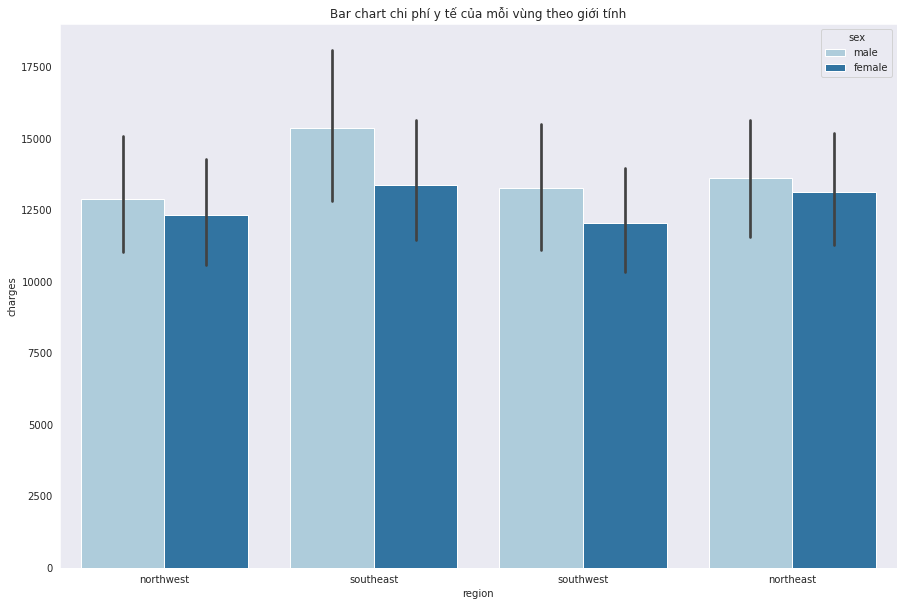
\includegraphics[width=1\textwidth]{images/bar_chart_medical_charges_region_sex.png}
		\caption{Chi phí y tế của mỗi vùng theo giới tính}
		\label{fig:writing-thesis-bar-chart-medical-charges-region-sex}
	\end{figure}
	\textbf{Nhận xét:} 
	\begin{itemize}
		\item Xét chi phí y tế là gần như tương đương nhau. Chi phí y tế của nam giới cao hơn hẳn so với nữ giới, ta có thể suy luận rằng lượng người khám và chữa bệnh là nam giới nhiều hơn nữ giới. Và điều này xảy ra ở mọi khu vực và nổi bật hơn ở Đông Nam và Tây Nam.
		\item Các cột chưa có nhiều sự chênh lệch đáng kể. Do đó, nhóm nhận định rằng đặc trưng \textbf{giới tính} có ít sự ảnh hưởng đến chi phí y tế theo từng vùng.
	\end{itemize}
	
	\subsection{6. Phân tích mối quan hệ chi phí y tế - vùng - tình trạng hút thuốc}
	\qquad Xét đặc trưng tình trạng hút thuốc và sự ảnh hưởng của nó đến chi phí y tế cá nhân theo từng vùng được nhóm trực quan bằng biểu đồ cột dưới đây.
	
	Dữ liệu được chọn là chi phí y tế theo trục tung, trục hoành biểu diễn vùng dân cư, mỗi vùng dân cư gồm hai cột: có - không hút thuốc
	\begin{figure}[H]
		\centering
		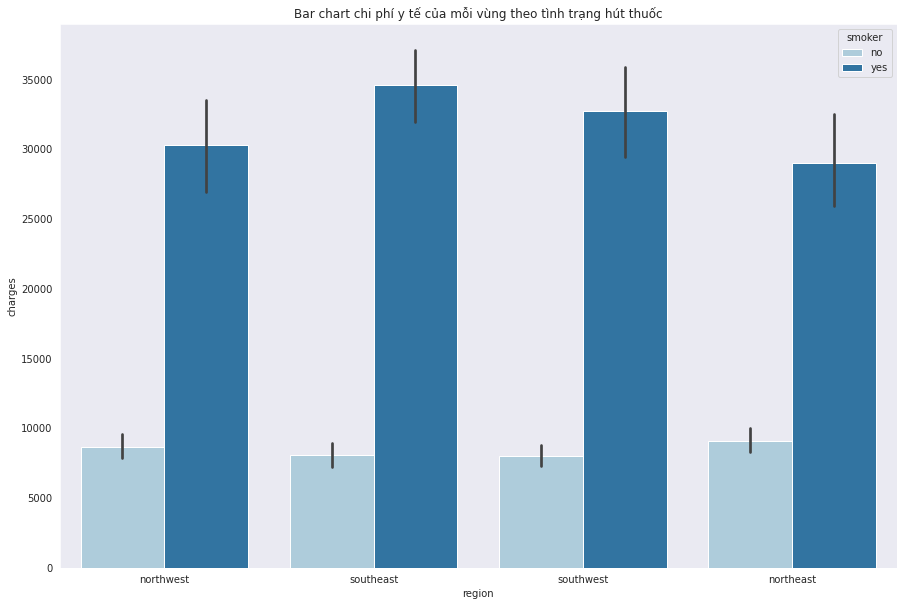
\includegraphics[width=1\textwidth]{images/bar_chart_medical_charges_region_smoker.png}
		\caption{Chi phí y tế của mỗi vùng theo tình trạng hút thuốc}
		\label{fig:writing-thesis-bar-chart-medical-charges-region-smoker}
	\end{figure}
	\textbf{Nhận xét:} 
	\begin{itemize}
		\item Xét ở mỗi vùng dân cư, số lượng người có hút thuốc cao hơn khoảng 3 lần so với người không hút.
		\item Ở khu vực miền Bắc lượng người hút thuốc thấp hơn so với miền Nam.
		\item Đồng thời ở khu vực miền Bắc lượng người không hút thuốc lớn hơn so với miền Nam. => tỉ lệ người không hút thuốc so với hút thuốc ở miền Bắc vượt trội với Miền Nam.
		\item Nhóm nhận định đặc trưng tình trạng hút thuốc là một trong những đặc trưng có sự ảnh hưởng tương đối lớn đối với chi phí y tế cá nhân.
	\end{itemize}

	\subsection{7. Phân tích mối quan hệ chi phí y tế - vùng - số lượng trẻ con/ người phụ thuộc}
	\qquad Xem xét đặc trưng số lượng trẻ con/ người phụ thuộc và sự ảnh hưởng của nó đến chi phí y tế cá nhân theo từng vùng được nhóm trực quan bằng biểu đồ cột dưới đây.
	
	Dữ liệu được chọn là chi phí y tế theo trục tung, trục hoành biểu diễn vùng dân cư, mỗi vùng dân cư gồm sáu cột: 0, 1, 2, 3, 4, 5 tương ứng với số lượng trẻ em/ người phụ thuộc
	\begin{figure}[H]
		\centering
		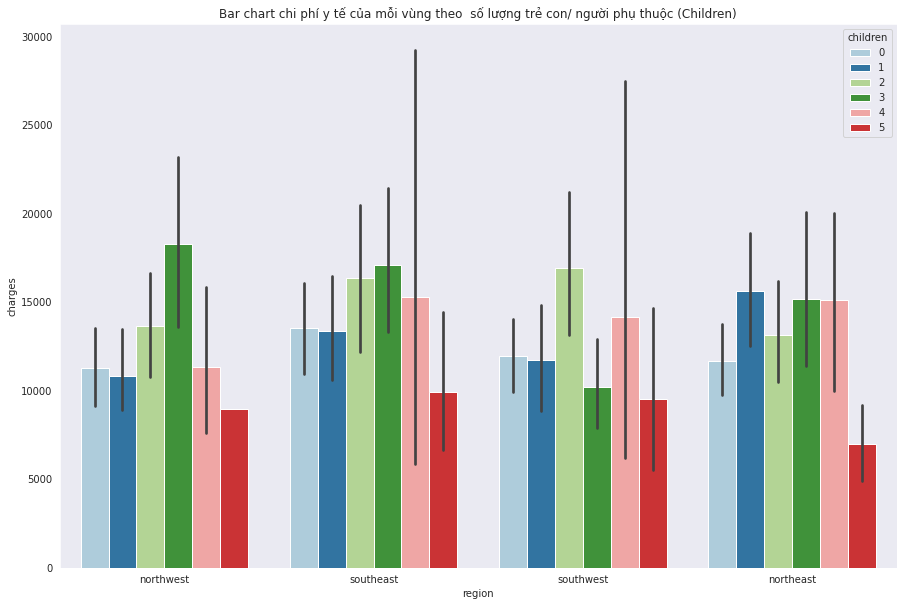
\includegraphics[width=1\textwidth]{images/bar_chart_medical_charges_region_children.png}
		\caption{Chi phí y tế của mỗi vùng theo số lượng trẻ con/ người phụ thuộc}
		\label{fig:writing-thesis-bar-chart-medical-charges-region-children}
	\end{figure}
	\textbf{Nhận xét:} 
	\begin{itemize}
		\item Nhìn chung chi phí y tế cá nhân ở người có 3 đứa trẻ đứng cao ngoại trừ vùng dân cư Tây Nam. 
		\item Chi phí y tế cá nhân ở người có 5 đứa trẻ ở mọi khu vực là thấp nhất. Điều này có nghĩa là ở đất nước này, khi có nhiều trẻ em/ người phụ thuộc người ta thường phải chi tiêu chặt chẽ hơn, tầng lớp người này có thể là người thu nhập trung bình khá, trung bình, nghèo do đó điều kiện không cho phép họ chi quá nhiều vào Y tế.
		\item Chi phí y tế cá nhân ở người không có trẻ em/ người phụ thuộc tương đối cao, cao hơn mức những người có 5 đứa trẻ/ người phụ thuộc.
		\item Nhóm nhận định đặc trưng số lượng trẻ con/ người phụ thuộc là một đặc trưng có ảnh hưởng tương đối ít đối với chi phí y tế cá nhân.
	\end{itemize}
	
	\subsection{8. Phân tích mối quan hệ giữa chi phí y tế và tuổi nhóm theo tình trạng hút thuốc}
	\qquad Xem xét mô hình tuyến tính (Linear Model) giữa  chi phí y tế và tuổi nhóm theo tình trạng hút thuốc
	
	Do hai đặc trưng chi phí y tế và tuổi là hai đại lượng liên tục nên dùng biểu đồ linear model trực quan quan hệ giữa chúng.
	
	Việc phân lớp theo đặc trưng tình trạng hút thuốc do đặc trưng này được nhóm nhận định là có ảnh hưởng khá lớn đối với chi phí y tế cá nhân
	\begin{figure}[H]
		\centering
		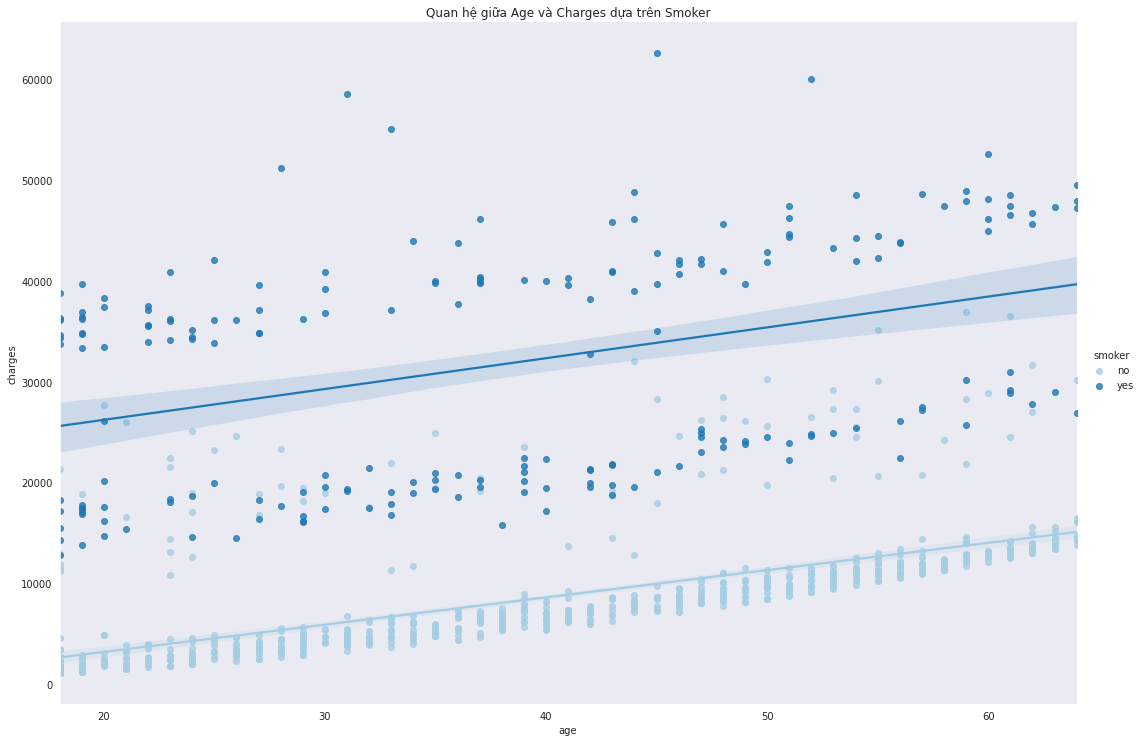
\includegraphics[width=1\textwidth]{images/age_charges_by_smoker.png}
		\caption{Quan hệ giữa Age và Charges dựa trên Smoker}
		\label{fig:writing-thesis-linear-model-medical-charges-age-group-smoker}
	\end{figure}
	\textbf{Nhận xét:} 
	\begin{itemize}
		\item Chi phí y tế của người hút thuốc cao hơn so với người không hút thuốc khoảng 23000.
		\item Chi phí y tế sẽ tăng dần đều theo số tuổi của người bệnh dù có hút thuốc hay không. => số tiền viện phí tăng thêm cần bỏ ra khi khám phụ thuộc vào tuổi, hút thuốc sẽ tăng thêm số tiền cố định thay vì tỉ lệ tăng dần.
	\end{itemize}

	\subsection{9. Phân tích mối quan hệ giữa chi phí y tế và chỉ số BMI nhóm theo tình trạng hút thuốc}
	\qquad Xem xét mô hình tuyến tính (Linear Model) giữa  chi phí y tế và chỉ số BM nhóm theo tình trạng hút thuốc
	
	Do hai đặc trưng chi phí y tế và chỉ số BM là hai đại lượng liên tục nên dùng biểu đồ linear model trực quan quan hệ giữa chúng.
	
	Việc phân lớp theo đặc trưng tình trạng hút thuốc do đặc trưng này được nhóm nhận định là có ảnh hưởng khá lớn đối với chi phí y tế cá nhân
	\begin{figure}[H]
		\centering
		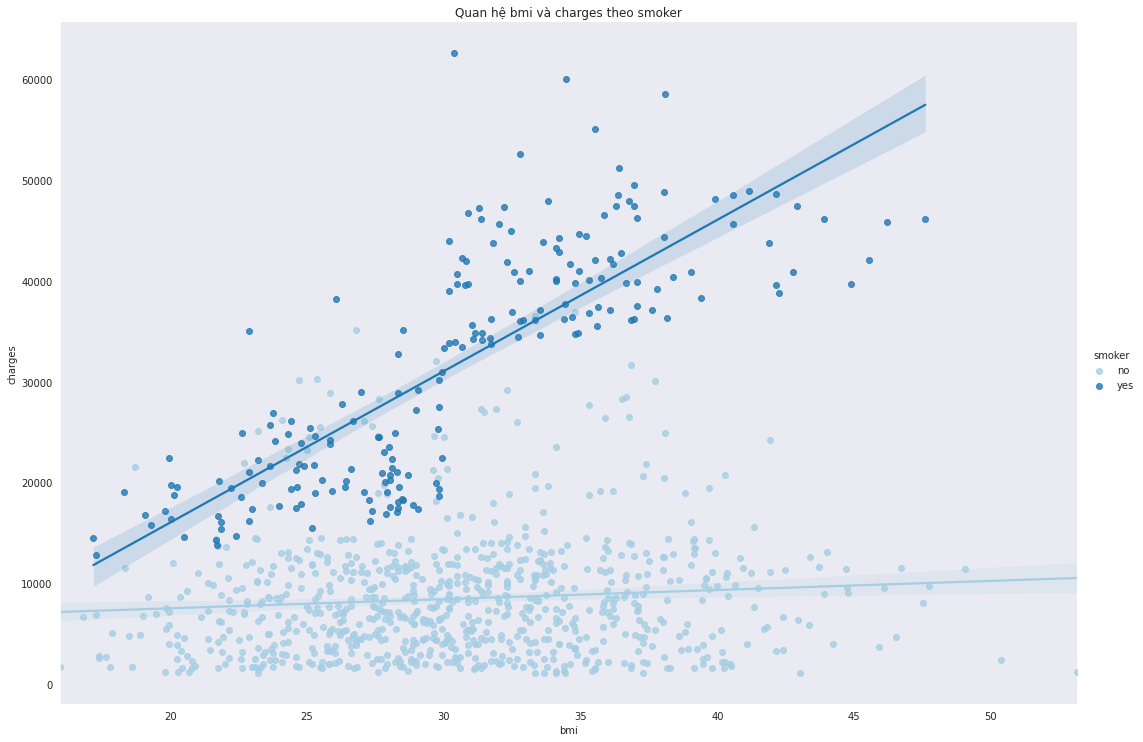
\includegraphics[width=1\textwidth]{images/bmi_charges_by_smoker.png}
		\caption{Quan hệ giữa Bmi và Charges dựa trên Smoker}
		\label{fig:writing-thesis-linear-model-medical-charges-bmi-group-smoker}
	\end{figure}
	\textbf{Nhận xét:} 
	\begin{itemize}
		\item Biểu đồ cho ta thấy số tiền viện phí khi không hút thuốc sẽ ổn định bất kể số bmi.
		\item Chi phí y tế của người không hút thuốc tăng với tỉ lệ cực thấp nếu không hút thuốc.
		\item Chi phí y tế của người hút thuốc sẽ tăng cao tỉ lệ thuận với bmi.
		\item Ở người hút thuốc tỉ lệ người có bmi thấp cao hơn so với ở người không hút.
	\end{itemize}

	\subsection{10. Phân tích  mối quan hệ giữa chi phí y tế và số lượng trẻ con/ người phụ thuộc nhóm theo tình trạng hút thuốc}
	\qquad Xem xét mô hình tuyến tính (Linear Model) giữa  chi phí y tế và số lượng trẻ con/ người phụ thuộc nhóm theo tình trạng hút thuốc
	
	Do hai đặc trưng chi phí y tế và số lượng trẻ con/ người phụ thuộc là hai đại lượng liên tục nên dùng biểu đồ linear model trực quan quan hệ giữa chúng.
	
	Việc phân lớp theo đặc trưng tình trạng hút thuốc do đặc trưng này được nhóm nhận định là có ảnh hưởng khá lớn đối với chi phí y tế cá nhân
	\begin{figure}[H]
		\centering
		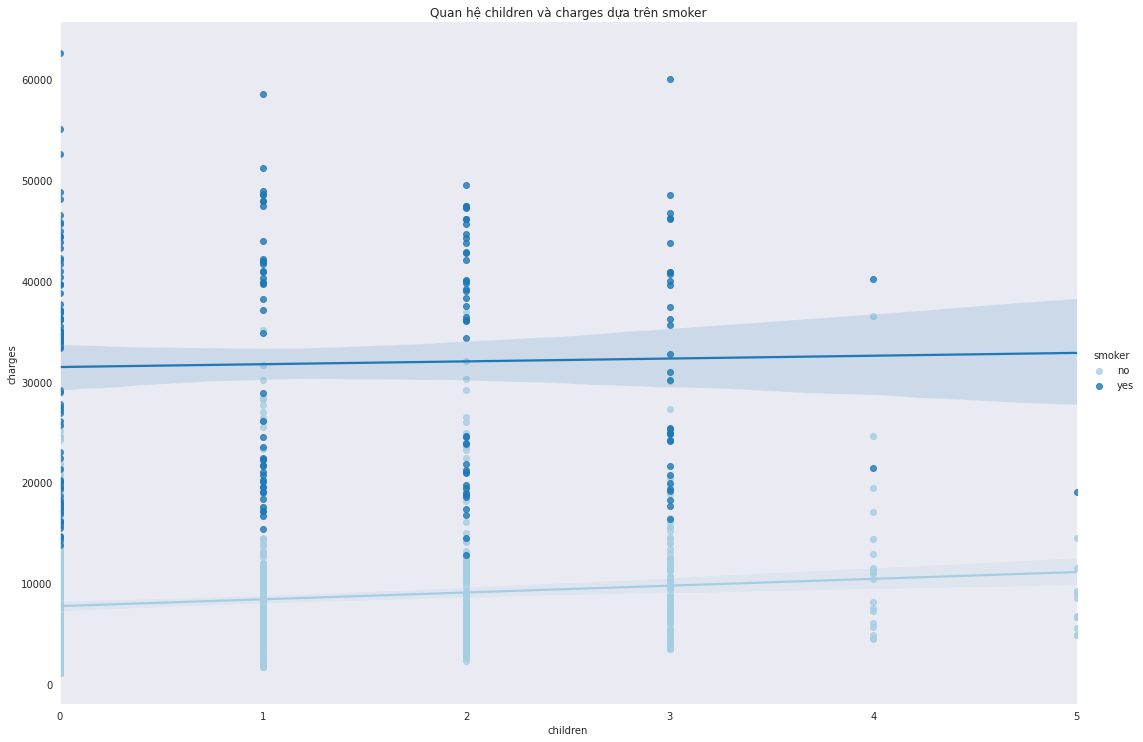
\includegraphics[width=1\textwidth]{images/children_charges_by_smoker.png}
		\caption{Quan hệ giữa Children và Charges dựa trên Smoker}
		\label{fig:writing-thesis-linear-model-medical-charges-children-group-smoker}
	\end{figure}
	\textbf{Nhận xét:} 
	\begin{itemize}
		\item
	\end{itemize}

	\subsection{11. Kết luận - Suy diễn}
	
	\section{3. Cài đặt thuật toán Máy học}
	
	\subsection{1. Lựa chọn thuật toán Máy học}
	\qquad Vấn đề đặt ra, dựa trên những dự kiện (các biến, giả định rằng các biến này độc lập với nhau) về tuổi (age), giới tính (sex), bmi, số lượng trẻ em (children), vùng dân cư (region), ta có thể đưa ra dự đoán về giá trị của chi phí y tế cá nhân (biến phụ thuộc) một cách chính xác nhất có thể
	
	Trong Học có giám sát (Supervised Learning) được chia ra làm 2 dạng lớn là hồi quy (regression) và phân loại (classification) dựa trên tập dữ liệu mẫu - tập huấn luyện (training data). Đây là một bài toán có thể áp dụng Mô hình Tuyến tính và Phân tích Hồi quy
	
	\textbf{Nhắc lại về bài toán Phân tích Hồi quy}
	Giả sử rằng một kết quả một quá trình bất kỳ nào đó được đại diện bằng một biến ngẫu nhiên $Y$, $Y$ được gọi là biến phụ thuộc, phụ thuộc vào $k$ biến khác $X_1, X_2, ..., X_k$

	Giả sử, biến $Y$ có thể được biểu diễn dạng như sau:
	\begin{align*}
		Y = f(X_1, X_2, ..., X_k, \beta_1, \beta_2, ..., \beta_k) + \beta_0
	\end{align*}
	Hàm $f$ là một hàm lý tưởng, $\beta_1, \beta_2, ..., \beta_k$ thể hiện sự đóng góp của $X_1, X_2, ..., X_k$, giá trị $\beta_0$ thể hiện sự ngẫu nhiên giữa $Y$ với $X_1, X_2, ..., X_k$
	
	Mô hình hay quan hệ này được gọi là tuyến tính nếu nó tuyến tính với các tham số của nó và phi tuyến nếu nó không tuyến tính với các tham số của nó. Có nghĩa là, nếu tất cả đạo hàm $y$ theo từng biến tham số $\beta_1, \beta_2, ..., \beta_k$ độc lập với các tham số thì mô hình gọi là tuyến tính.
	
	\textbf{Mục tiêu của Phân tích Hồi quy} Việc xác định dạng tường minh của phương trình hồi quy là mục tiêu cuối cùng của phân tích hồi quy. Cuối cùng nó là một mối quan hệ tốt và hợp lệ giữa biến nghiên cứu và biến giải thích. Một phương trình hồi quy như vậy có thể được sử dụng cho một số mục đích. 
	
	Ví dụ, để xác định vai trò của bất kỳ biến giải thích nào trong mối quan hệ chung trong bất kỳ xây dựng chính sách nào, để dự báo các giá trị của biến phản hồi cho một tập hợp các giá trị nhất định của các biến giải thích. Phương trình hồi quy giúp hiểu được mối quan hệ qua lại của các biến giữa chúng.
	
	\textbf{Các bước thực hiện của Phân tích Hồi quy}
	\begin{itemize}
		\item Phát biểu bài toán/ vấn đề
		\item Lựa chọn những biến có liên quan đến bài toán
		\item Thu thập dữ liệu về những biến đã chọn có liên quan đến bài toán
		\item Đặc điểm kỹ thuật của mô hình
		\item Lựa chọn phương pháp để điều chỉnh dữ liệu
		\item Khớp mô hình
		\item Kiểm định và đánh giá mô hình
		\item Sử dụng (các) mô hình đã chọn cho giải pháp của vấn đề đã đặt ra.
	\end{itemize}

	\textbf{Đánh giá Phân tích Hồi quy}
	Các độ đo sử dụng trong việc đánh giá các mô hình Hồi quy trong bài lab
	\begin{itemize}
		\item Độ đo Mean Absolute Error được tính theo công thức:
		$$\text{MAE} = \frac{\sum_{i=1}^n|y_i-x_i|}{n}$$
		Độ đo này thường được sử dụng để đánh giá sự sai khác giữa mô hình dự đoán và tập dữ liệu kiểm tra trong các bài toán hồi quy. Chỉ số này càng nhỏ thì mô hình học máy càng chính xác.
		\item Mean squared error - MSE hay được biết là phép ước lượng trung bình của bình phương của sai số. MSE là moment bậc hai (về nguồn gốc) của sai số là moment bậc hai (về nguồn gốc) của sai số
		$$MSE = \frac{1}{n}\sum_{i=1}^{n}(Y_i - \hat{Y})^2$$
		\item Căn bậc 2 của trung bình bình phương sai số
		$$RMSE = \sqrt[2]{\frac{1}{n}\sum_{i=1}^{n}(Y_i - \hat{Y})^2}$$
		\item R2 (R Squared)
		$$R^2 = \frac{MSS}{TSS} = 1 - \frac{ESS}{TSS} = \frac{\sum(Y_i - \overline{Y})^2}{\sum(\hat{Y} - \overline{Y})^2} = 1 - \frac{\sum(Y_i - \hat{Y})^2}{\sum(\hat{Y} - \overline{Y})^2}$$
	\end{itemize}
	
	
	\subsection{2. Hồi quy Tuyến tính - Linear Regression}
	\subsubsection{Sklearn Hồi quy tuyến tính}
	\qquad Thông qua những dữ liệu, thuật toán và mô hình máy học đã được học, ta hy vọng sẽ đưa ra giá trị dự đoán về một quá trình nào đó một cách chính xác nhất (tương ứng với những biến mới). Thông thường những biến giá trị này có tính liên tục
	
	Tùy theo số lượng biến mà mô hình có hình dạng khác nhau
	\begin{itemize}
		\item Với số lượng biến $r = 1$, mô hình sẽ có dạng một đường thẳng: $Y = \beta_0 + \beta_1X + \epsilon$
		\item Với số lượng biến $r = 2$, mô hình sẽ có dạng một mặt thẳng: $Y = \beta_0 + \beta_1X_2 + \beta_2X_2 + \epsilon$
		\item Với số lượng biến $r > 2$, mô hình sẽ có dạng một siêu phẳng
	\end{itemize}
	Một mô hình tuyến tính dự đoán kết quả bằng cách tính tổng trọng số của các đặc trưng đầu vào (hay các biến độc lập). 
	$$ \hat{y}=w_0+w_1x_1+w_2x_2+...+w_nx_n $$
	\begin{itemize}
		\item $\hat{y}$ là giá trị dự đoán.
		\item $n$ là số lượng đặc trưng.
		\item $x_i$ là giá trị đặc trưng thứ $i$.
		\item $w_j$ là tham số thứ $j$ của mô hình.
	\end{itemize}
	$$\hat{y}=h_{\mathbf{w}}\left(\mathbf{x}\right)=\mathbf{w}^{T}\cdot\mathbf{x}$$
	\begin{itemize}
		\item $\mathbf{w}$ \textbf{vector trọng số} của mô hình (bao gốm cả $w_0$ và các trọng số đặc trưng $w_1,w_2,...w_n$).
		\item $\mathbf{w}^T$ là chuyển vị của $\mathbf{w}$ (vector hàng thay vì vector cột).
		\item $\mathbf{x}$ là \textbf{vector đầu vào} của các mẫu dữ liệu, bao gồm $x_0$ đến $x_n$, với $x_0$ luôn có giá trị là 1.
		\item $\mathbf{w}^{T}\cdot\mathbf{x}$ là tích vô hướng của 2 vector $\mathbf{w}^T$ và $\mathbf{x}$.
		\item $h_{\mathbf{w}}$ là hàm giả thiết, biểu diễn bằng các tham số $\mathbf{w}$.
	\end{itemize}

	\textbf{Các bước thực hiện} Hồi quy tuyến tính với thư viện \textbf{Sklearn}
	\begin{itemize}
		\item \textbf{Chuẩn bị dữ liệu}
		\begin{figure}[H]
			\centering
			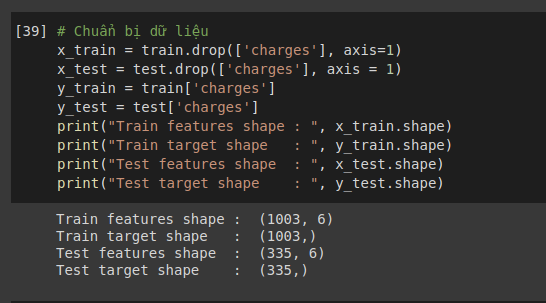
\includegraphics[width=0.75\textwidth]{images/linear_reg/linear_reg_data_preparation.png}
		\end{figure}
		Tập dữ liệu huấn luyện, tập dữ liệu kiểm tra được đọc từ hai tập tin được cung cấp là train.csv và test.csv bằng Pandas, có dạng là data frame
		
		\item \textbf{Khởi tạo mô hình}
		\begin{figure}[H]
			\centering
			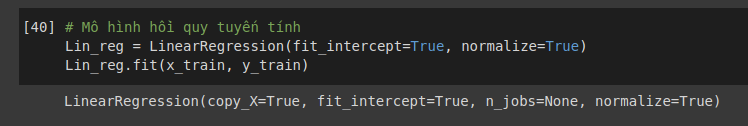
\includegraphics[width=0.75\textwidth]{images/linear_reg/linear_reg_init.png}
		\end{figure}
		Sklearn sử dụng phương pháp bình phương tối tiểu để ước lượng tham số cho mô hình. LinearRegression khớp dữ liệu với các hệ số $w = (w1,…, wp)$ để giảm thiểu tổng bình phương còn lại giữa các mục tiêu được quan sát trong tập dữ liệu và các mục tiêu được dự đoán bằng phép gần đúng tuyến tính.
		Các tham số khi khởi tạo hàm LinearRegression
		\begin{itemize}
			\item fit\_intercept: 
			\item normalize:
			\item copy\_X:
			\item n\_jobs: 
			\item positive:
		\end{itemize}
		
		\item Hệ số của các đặc trưng, hệ số chặn trong mô hình regression của dữ liệu, điểm số trên tập test
		\begin{figure}[H]
			\centering
			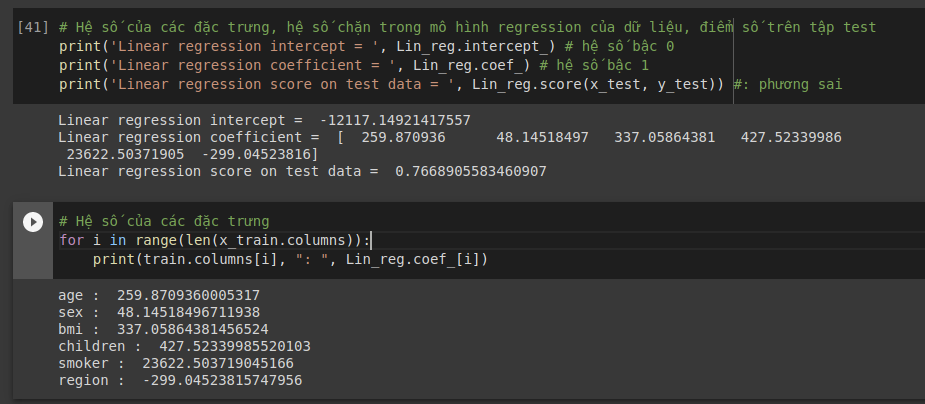
\includegraphics[width=0.75\textwidth]{images/linear_reg/linear_reg_res.png}
		\end{figure}
		Giá trị $\text{Linear regression intercept} =  -12117.149214175606$ tương ứng hệ số $\beta_0$ của mô hình, nó có ý nghĩa là giá trị chặn của mô hình (dễ hiểu là số b của đường thẳng y=ax + b)
		
		Các giá trị Linear regression coefficient = [259.870936,48.14518497,337.05864381,427.52339986, 23622.50371905,-299.04523816] là các hệ số tương ứng với các đặc trưng của dữ liệu, lần lượt 
		\begin{itemize}
			\item age :  259.87093600053163
			\item sex :  48.145184967129666
			\item bmi :  337.05864381456627
			\item children :  427.5233998551999
			\item smoker :  23622.503719045195
			\item region :  -299.04523815748104
		\end{itemize}
		
		Giá trị $\text{Linear regression score on test data} =  0.7668905583460909 $, có ý nghĩa là hệ số xác định $R^2$ của dự đoán trên tập dữ liệu kiểm tra.
		
		Hệ số $R^2$ được định nghĩa bằng biểu thức $\left(1 - \frac{u}{v}\right)$. Trong đó:
		\begin{itemize}
			\item $u$ là tổng bình phương phần dư (Residual Sum of Squares - RSS):((y\_true - y\_pred) ** 2).sum()
			\item $v$ là tổng độ lệch bình phương của toàn bộ đặc trưng (Total Sum of Squares - TSS): ((y\_true - y\_true.mean()) ** 2).sum()
			\item Giá trị lớn nhất có thể là dương 1.0, $R^2$ có thể âm. Khi giá trị $R^2$ bằng 0, mô hình luôn dự đoán giá trị kỳ vọng của y
		\end{itemize}
		\item \textbf{Dự đoán}
		\begin{itemize}
			\item Trên tập huấn luyện
			\begin{figure}[H]
				\centering
				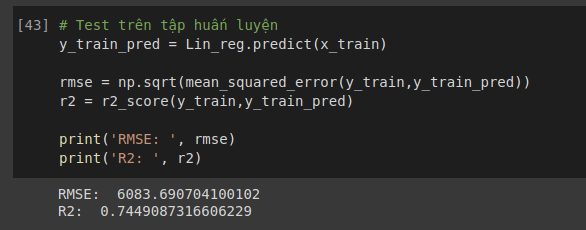
\includegraphics[width=0.75\textwidth]{images/linear_reg/linear_reg_predict_train.png}
			\end{figure}
			Nhóm tính toán hai thông số để đánh giá mô hình trên tập huấn luyện
			\begin{itemize}
				\item RMSE (sai số bình phương trung bình gốc - Root Mean Squares Error): 6083.690704100102
						
				\item $R^2$: 0.7449087316606229
			\end{itemize}
			\item Trên tập kiểm tra
			\begin{figure}[H]
				\centering
				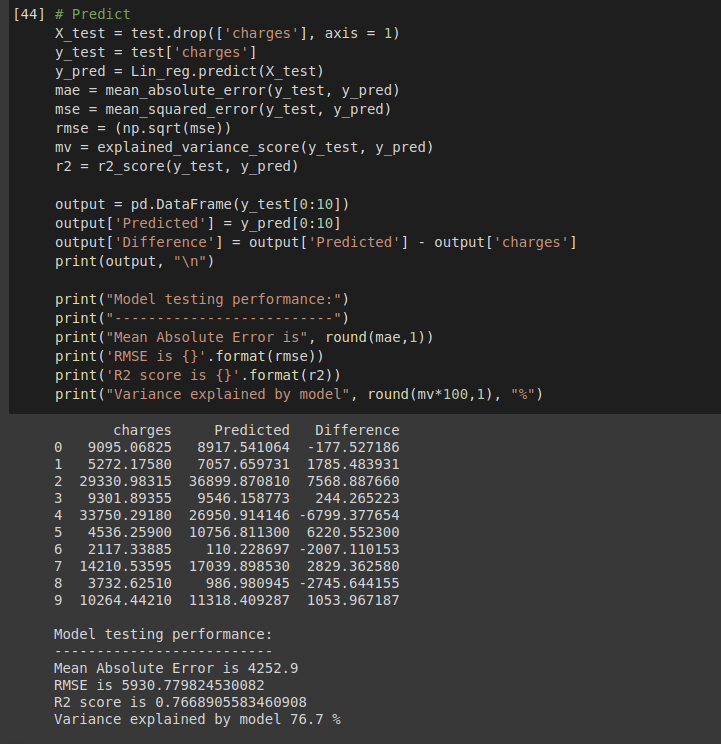
\includegraphics[width=0.75\textwidth]{images/linear_reg/linear_reg_predict_test.png}
			\end{figure}
			Hiển thị bảng đối sánh kết quả thực và kết quả dự đoán, đánh giá thông qua các độ đo:
			\begin{itemize}
				\item Mean Absolute Error đạt 4252.9				
				\item RMSE đạt 5930.779824530081
				\item R2 score đạt 0.7668905583460909, gần về 1.0
				\item Variance explained by model 76.6909\%
			\end{itemize}
		\end{itemize}
		\item \textbf{Trực quan hóa kết quả}
		\begin{figure}[H]
			\centering
			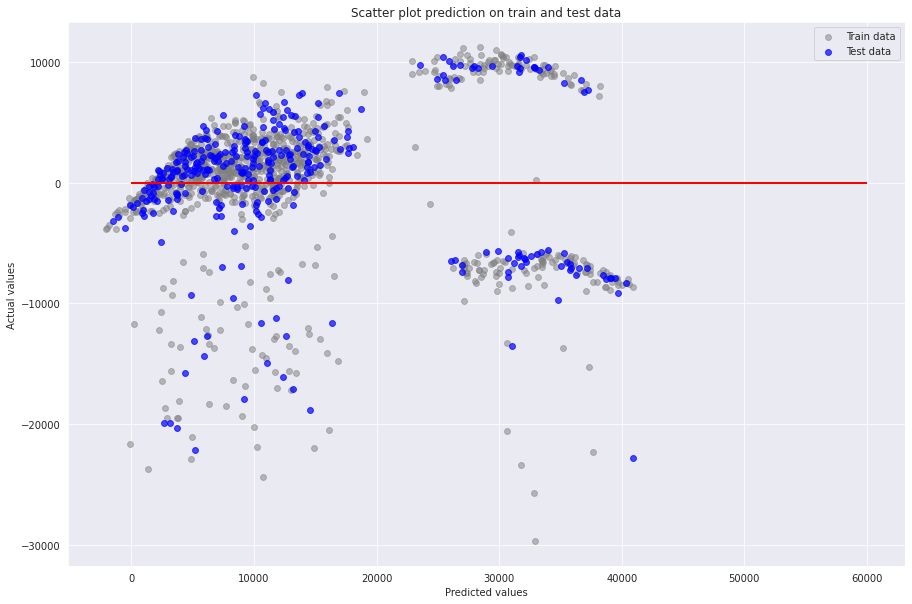
\includegraphics[width=0.85\textwidth]{images/linear_reg/linear_reg_plot.png}
		\end{figure}	
	\end{itemize}
	\subsubsection{Nhận xét}
	\begin{itemize}
		\item Mô hình hoàn thành được mục tiêu đề ra là dự đoán được chi phí y tế cá nhân với giá trị $R^2$ tương đối cao 0.76, giải thích phương sai đat 76.7\%
		\item Công thức Linear Regression: $\text{predict} = \text{intercept} + \text{slopeAge} * \text{dataAge} + \text{slopeSex} * \text{dataSex} + \text{slopeBMI} * \text{dataBMI} + ...$
		\item Dựa vào bộ train data, Linear Regression tính toán với bình phương phương sai thấp nhất của dữ liệu so với dữ liệu cần dự đoán, từ đó tìm hệ số slope của mỗi dữ liệu đối với kết quả cần được dự đoán (coefficient). từ đó tìm ra được chi phí phù hợp khi từng loại dữ liệu được đặt ra.
	\end{itemize}
	\textbf{Ưu điểm - nhược điểm của Hồi quy tuyến tính}
	\begin{itemize}
		\item Ưu điểm
		\begin{itemize}
			\item \textbf{Mô hình đơn giản:} Mô hình hồi quy tuyến tính là phương trình đơn giản nhất sử dụng để biểu diễn mối quan hệ giữa nhiều biến dự báo và biến dự đoán.
			\item \textbf{Hiệu quả về mặt tính toán:} Tốc độ lập mô hình của hồi quy tuyến tính nhanh vì nó không yêu cầu tính toán phức tạp và chạy dự đoán nhanh khi lượng dữ liệu lớn.
			\item \textbf{Khả năng diễn giải của đầu ra:} Diễn giải được ảnh hưởng tương đối của một hoặc nhiều biến dự báo đến giá trị dự đoán khi các yếu tố dự báo độc lập với nhau. Có thể thể hiện sự thay đổi nào trong biến dự báo gây ra thay đổi nào trong biến dự đoán hoặc biến mục tiêu
		\end{itemize}
		\item Nhược điểm
		\begin{itemize}
			\item \textbf{Quá đơn giản:} Mô hình hồi quy tuyến tính quá đơn giản để nắm bắt được độ phức tạp của thế giới thực.
			\item \textbf{Giả định tuyến tính:} Hồi quy tuyến tính đưa ra giả định mạnh mẽ rằng có các biến Dự đoán (độc lập) và Dự đoán (phụ thuộc) có quan hệ tuyến tính với nhau, điều này không hợp lý, vì trong thế giới thực, có rất nhiều mối quan hệ không có sự phự thuộc tuyến tính (phụ thuộc phi tuyến).
			\item \textbf{Bị ảnh hưởng nghiêm trọng bởi các điểm ngoại lai:} Các điểm ngoại lệ có thể có ảnh hưởng lớn đến kết quả đầu ra.
			\item \textbf{Tính độc lập của các biến:} Giả định rằng các biến dự báo không tương quan với nhau, điều này hiếm (hoặc không có) trong thực tế.
			\item Hồi quy tuyến tính chỉ xem xét mối quan hệ giữa giá trị trung bình của biến dự đoán/ phụ thuộc và các biến dự đoán/ độc lập và giả định phương sai không đổi xung quanh giá trị trung bình.
		\end{itemize}
	\end{itemize}
	\subsection{3. Hồi quy Ridge - Ridge Regression}
	\subsubsection{Hồi quy Ridge cơ bản}
	Giả sử rằng X và Y đã được căn giữa, do đó không cần một số hạng không đổi trong hồi quy:
	\begin{itemize}
		\item X là ma trận kích thước $n \times p$
		\item Y là vector có n phần tử
	\end{itemize}
	Hoerl và Kennard (1970) nhận thấy rằng sự không ổn định tiềm ẩn trong ước lượng LS
	$$\hat{\beta} = (X'X)^{-1}X'Y$$
	có thể được cải thiện bằng cách thêm một giá trị không đổi nhỏ $\lambda$ vào các phần tử trên đường chéo của ma trận $X'X$ trước khi nghịch đảo của nó.
	
	Và kết quả là có được một ước lượng hồi quy Ridge như sau
	$$\hat{\beta}_{\text{ridge}} = (X'X + \lambda I_p)^{-1}X'Y$$
	Hồi quy Ridge đặt một dạng ràng buộc cụ thể lên các tham số $\beta$, $\hat{\beta}_{\text{ridge}}$ sẽ được chọn sao cho làm tối tiểu tổng bình phương giá trị bị phạt
	$$\sum{i=1}^{n}\left(y_i - \sum_{j=1}^p(x_{ij}\beta_{j})\right)^2 + \lambda\sum_{j=1}^{p}\beta_j^2$$
	tương đương với việc giảm thiểu 
	$$\sum{i=1}^{n}\left(y_i - \sum_{j=1}^p(x_{ij}\beta_{j})\right)^2$$ phụ thuộc vào một số thực dương $c > 0$ mà $\sum_{j=1}^{p}\beta_j^2 < c$
	\begin{figure}[H]
		\centering
		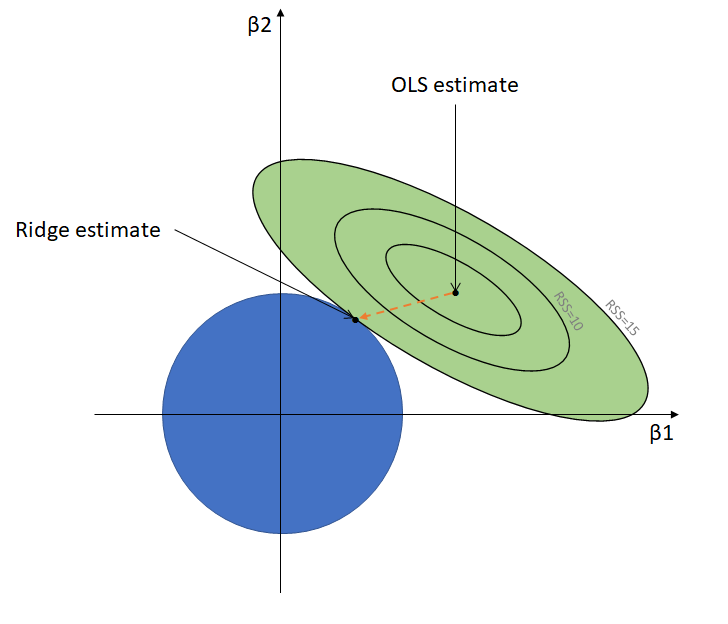
\includegraphics[width=0.65\textwidth]{images/ridge_reg/ridge_geometric.png}
	\end{figure}
	\begin{figure}[H]
		\centering
		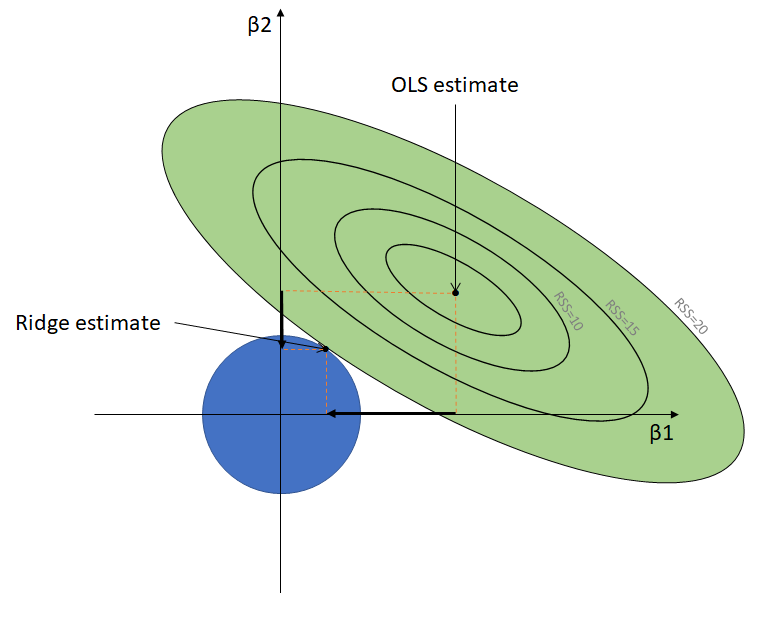
\includegraphics[width=0.65\textwidth]{images/ridge_reg/ridge_geometric_2.png}
	\end{figure}
	\subsubsection{Sklearn Hồi quy Ridge}
	Các bước thực hiện Hồi quy Ridge với thư viện Sklearn
	\begin{itemize}
		\item \textbf{Chuẩn bị dữ liệu}
		\begin{figure}[H]
			\centering
			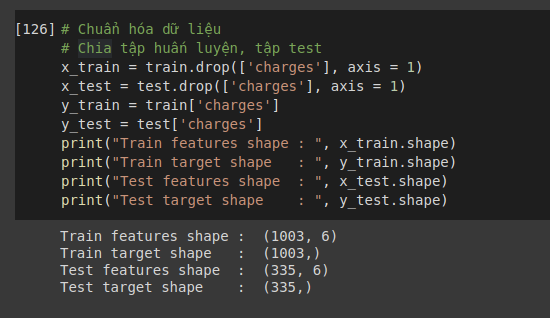
\includegraphics[width=0.85\textwidth]{images/ridge_reg/ridge_reg_data_preparation.png}
		\end{figure}
		Tập dữ liệu huấn luyện, tập dữ liệu kiểm tra được đọc từ hai tập tin được cung cấp là train.csv và test.csv bằng Pandas, có dạng là data frame
		
		\item \textbf{Chọn giá trị alpha tối ưu}
		\begin{figure}[H]
			\centering
			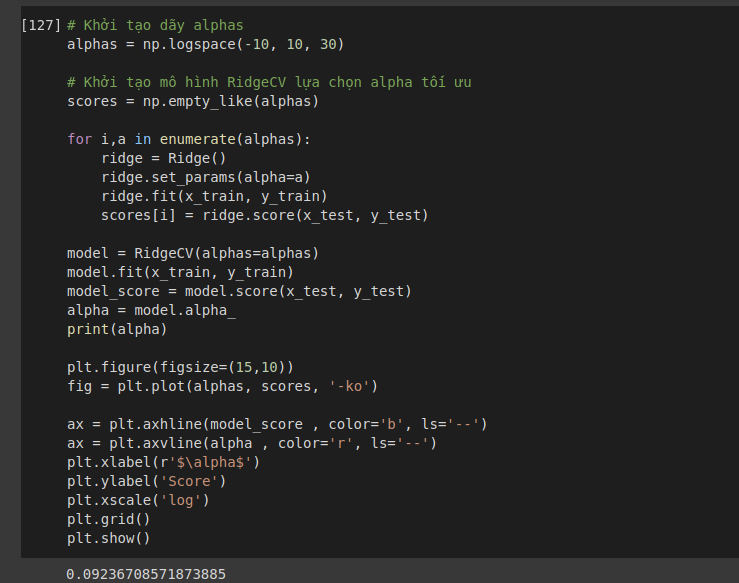
\includegraphics[width=0.85\textwidth]{images/ridge_reg/ridge_reg_optimal_alpha.png}
		\end{figure}
		Do tập huấn luyện khá nhỏ, khoảng 1000 mẫu, nhóm quyết định chọn alpha tối ưu bằng cách thử nghiệm, tạo logspace bằng Numpy trong khoảng [-10, 10], khởi tạo 30 giá trị, fit lần lượt các giá trị alpha đó thông qua lớp RidgeCV Sklearn để chọn alpha tối ưu.
		
		Hình bên dưới mô tả quá trình duyệt để chọn alpha, đường màu đỏ là giá trị alpha, đường màu xanh là điểm số mô hình trên tập kiểm tra.
		\begin{figure}[H]
			\centering
			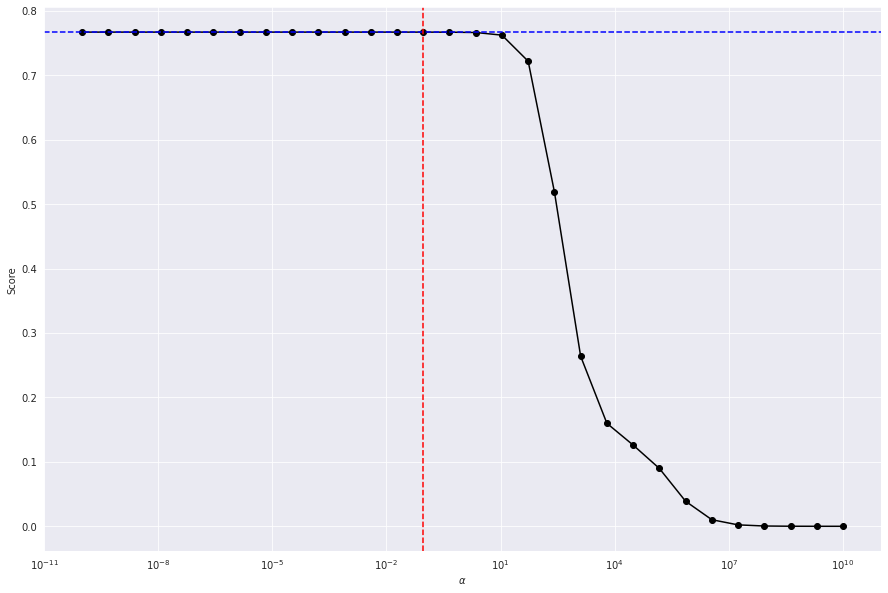
\includegraphics[width=0.85\textwidth]{images/ridge_reg/ridge_choose_alpha.png}
		\end{figure}
		
		\item \textbf{Khởi tạo và huấn luyện mô hình}
		\begin{figure}[H]
			\centering
			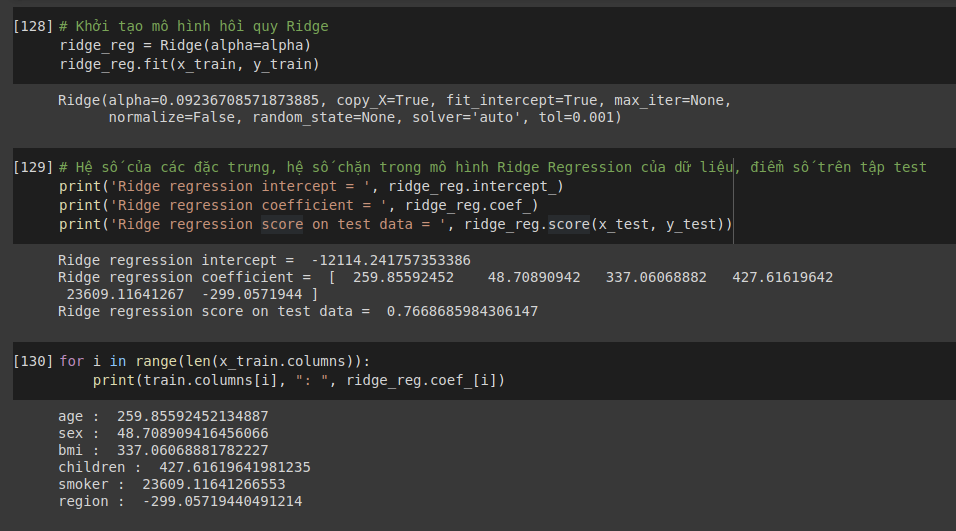
\includegraphics[width=0.85\textwidth]{images/ridge_reg/ridge_reg_init_training.png}
		\end{figure}
		\textbf{Khởi tạo mô hình} Các tham số khi dùng khởi tạo mô hình Ridge
		\begin{itemize}
			\item alpha: hệ số alpha cho mô hình
			\item fit\_intercept: Có khớp với chặn cho mô hình này hay không. Nếu được đặt thành false, sẽ không có đánh chặn nào được sử dụng trong quá trình tính toán
			\item normalize: Tham số này bị bỏ qua khi fit\_intercept được đặt thành False. Nếu True, các hồi quy X sẽ được chuẩn hóa trước khi hồi quy bằng cách trừ giá trị trung bình và chia cho l2-norm
			\item copy\_X: Nếu True thì X sẽ được copy, không thì X sẽ bị ghi đè
			\item max\_iter: Số lần lặp tối đa cho bộ giải gradient liên hợp
			\item tol: Làm tròn cho mô hình
			\item solver: chọn bộ tính toán cho mô hình
			\begin{itemize}
				\item auto - Tự động chọn quy trình tính toán
				\item svd - Singular Value Decomposition: sử dụng phép phân tích giá trị đơn lẻ của X để tính toán các hệ số Ridge.
				\item cholesky - sử dụng hàm scipy.linalg.solve tiêu chuẩn để nhận được một lời giải tối ưu
				\item sparse\_cg - sử dụng bộ giải gradient liên hợp như được tìm thấy trong scipy.sparse.linalg.cg. Là một thuật toán lặp lại, bộ giải này thích hợp hơn ‘cholesky’ đối với dữ liệu quy mô lớn
				\item lsqr - sử dụng dedicated regularized least-squares trong scipy.sparse.linalg.lsqr. Nó là nhanh nhất và sử dụng một thủ tục lặp đi lặp lại.
				\item sag - Stochastic Average Gradient descent: sử dụng Stochastic Average Gradient descent và 'saga' sử dụng phiên bản cải tiến, không bias có tên là SAGA. Cả hai phương pháp cũng sử dụng một thủ tục lặp lại và thường nhanh hơn các trình giải khác khi cả n\_samples và n\_features đều lớn
			\end{itemize}
			\item random\_state: Sử dụng khi dùng 'sag' hoặc 'saga' 
		\end{itemize}
		\item Dự đoán
		\begin{itemize}
			\item Trên tập huấn luyện
			\begin{figure}[H]
				\centering
				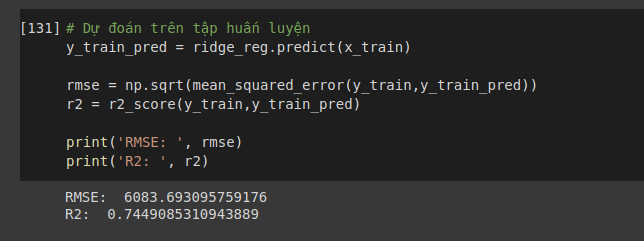
\includegraphics[width=0.85\textwidth]{images/ridge_reg/ridge_reg_predict_train.png}
			\end{figure}
		Hiệu quả trên tập huấn luyện được đánh giá bằng RMSE, R2 Score
		\begin{itemize}
			\item RMSE:  6083.693095759176
			\item R2:  0.7449085310943889, chỉ số này khá gần 1.0
		\end{itemize}
			\item Trên tập kiểm tra
			\begin{figure}[H]
				\centering
				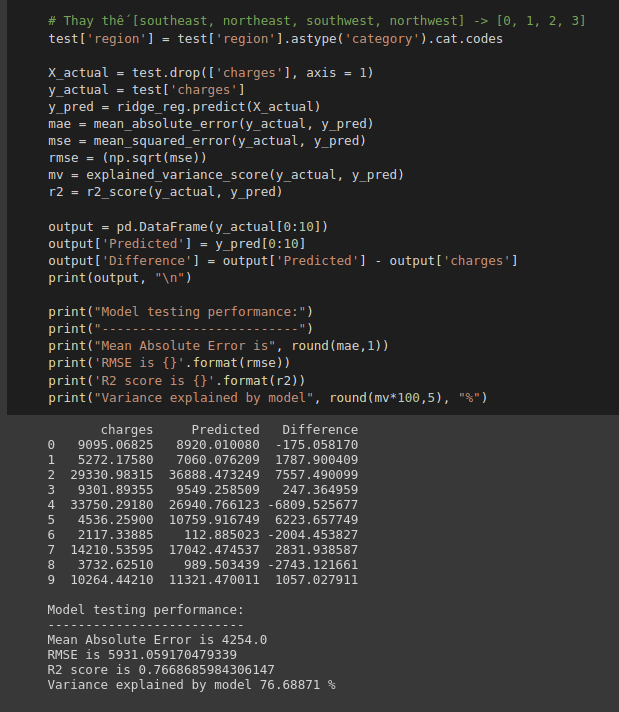
\includegraphics[width=0.85\textwidth]{images/ridge_reg/ridge_reg_predict_test.png}
			\end{figure}
			Hiển thị bảng đối sánh kết quả thực và kết quả dự đoán, đánh giá thông qua các độ đo:
			\begin{itemize}
				\item Mean Absolute Error is 4254.0
				\item RMSE is 5931.059170479339
				\item R2 score is 0.7668685984306147
				\item Variance explained by model 76.68871\%
			\end{itemize}
		\end{itemize}
		\item \textbf{Trực quan kết quả dự đoán}
		\begin{figure}[H]
			\centering
			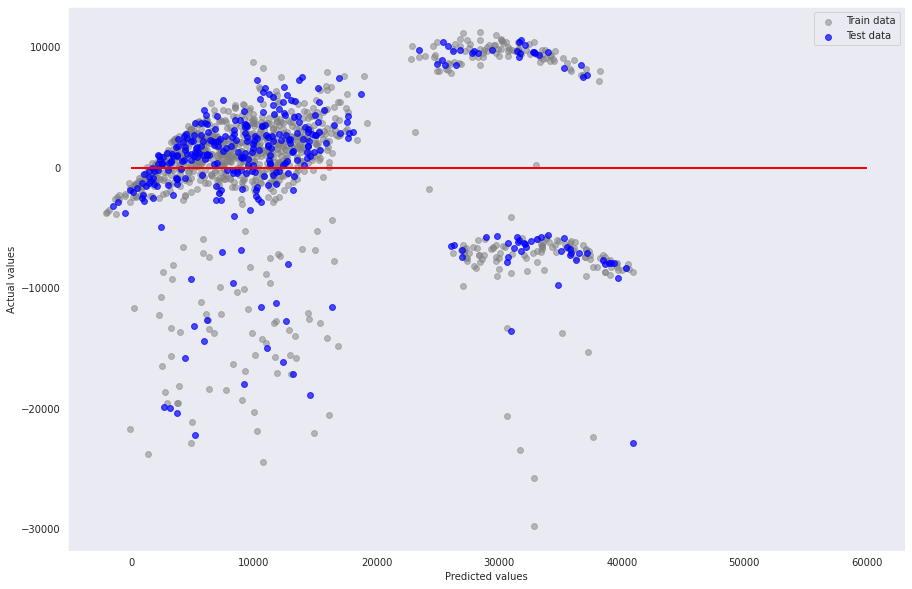
\includegraphics[width=0.85\textwidth]{images/ridge_reg/ridge_reg_plot.png}
		\end{figure}
	\end{itemize}
	\subsubsection{Nhận xét}
	\begin{itemize}
		\item Tương tự với Linear Regression, Ridge cũng tìm hệ dữ liệu với phương sai thấp nhất.
		
		\item Ridge tìm ra hệ số bias lớn hơn so với Linear để giảm hoặc tăng tính ảnh hưởng của từng loại dữ liệu lên kết quả được predict.
		\item So sánh Ridge và Linear Regression
		\begin{itemize}
			\item $\text{Linear tính toán predict} = \text{tổng bình phương phương sai thấp nhất với slope} * \text{data}$
			\item $\text{Ridge tính toán predict} = \text{tổng bình phương phương sai thấp nhất} + \lambda \times \text{slope}^2.$
		\end{itemize}
	\end{itemize}
	\textbf{Ưu điểm và nhược điểm của mô hình Hồi quy Ridge - Ridge Regression}
	\begin{itemize}
		\item Ưu điểm:
		\item Nhược điểm:
	\end{itemize}
	\subsection{4. Hồi quy Lasso - Lasso Regression}
	\subsubsection{Hồi quy Lasso cơ bản}
	\subsubsection{Sklearn Hồi quy Lasso}
	Các bước thực hiện Hồi quy Lasso với thư viện Sklearn
	\begin{itemize}
		\item Chuẩn bị dữ liệu
		\begin{figure}[H]
			\centering
			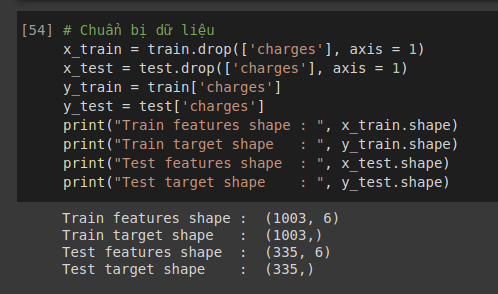
\includegraphics[width=0.75\textwidth]{images/lasso_reg/lasso_data_preparation.png}
		\end{figure}
		Tập dữ liệu huấn luyện, tập dữ liệu kiểm tra được đọc từ hai tập tin được cung cấp là train.csv và test.csv bằng Pandas, có dạng là data frame
		\item Chọn alpha
		\begin{figure}[H]
			\centering
			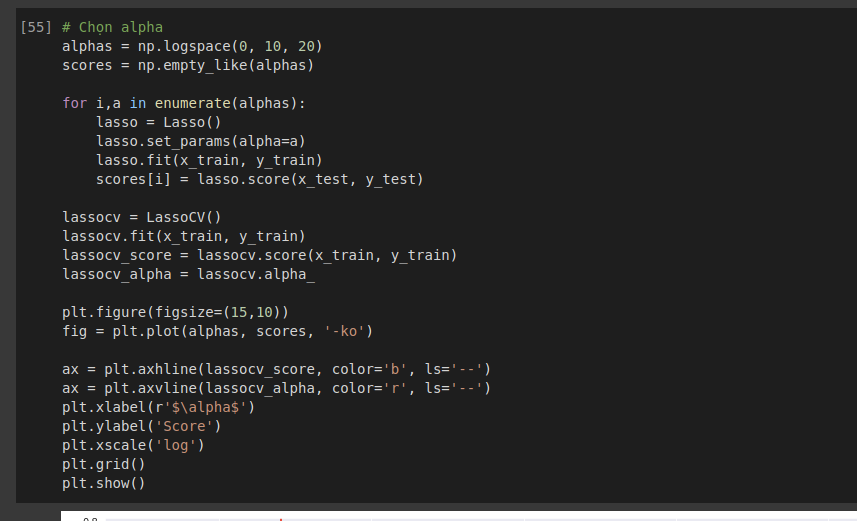
\includegraphics[width=0.75\textwidth]{images/lasso_reg/lasso_reg_choose_alpha.png}
		\end{figure}
		Do tập huấn luyện khá nhỏ, khoảng 1000 mẫu, nhóm quyết định chọn alpha tối ưu bằng cách thử nghiệm, tạo logspace bằng Numpy trong khoảng [-10, 10], khởi tạo 30 giá trị, fit lần lượt các giá trị alpha đó thông qua lớp LassoCV Sklearn để chọn alpha tối ưu.
	
		Hình bên dưới mô tả quá trình duyệt để chọn alpha, đường màu đỏ là giá trị alpha, đường màu xanh là điểm số mô hình trên tập kiểm tra.
		\begin{figure}[H]
			\centering
			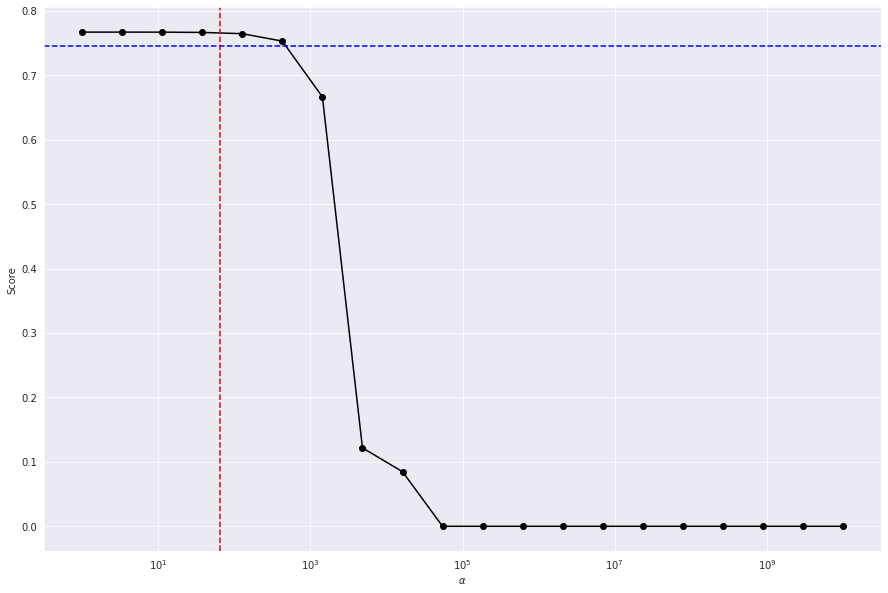
\includegraphics[width=0.75\textwidth]{images/lasso_reg/lasso_choose_alpha.png}
		\end{figure}
		\item Khởi tạo và fit mô hình
		\begin{figure}[H]
			\centering
			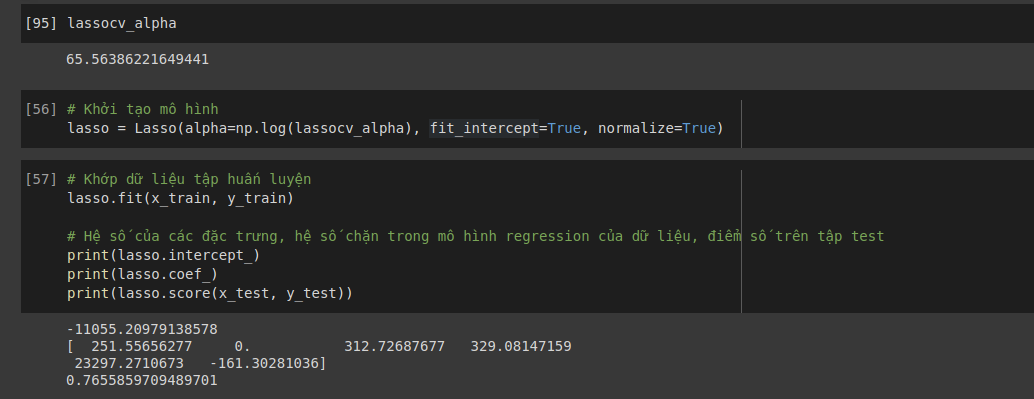
\includegraphics[width=0.75\textwidth]{images/lasso_reg/lasso_init_fit.png}
		\end{figure}
		\textbf{Khởi tạo mô hình} Các tham số khi dùng khởi tạo mô hình Lasso
		\begin{itemize}
			\item alpha
			\item fit\_intercept: Có khớp với chặn cho mô hình này hay không. Nếu được đặt thành false, sẽ không có đánh chặn nào được sử dụng trong quá trình tính toán
			\item normalize: Tham số này bị bỏ qua khi fit\_intercept được đặt thành False. Nếu True, các hồi quy X sẽ được chuẩn hóa trước khi hồi quy bằng cách trừ giá trị trung bình và chia cho l2-norm
			\item precompute
			\item copy\_X: Nếu True thì X sẽ được copy, không thì X sẽ bị ghi đè
			\item max\_iter: Số lần lặp tối đa cho bộ giải gradient liên hợp
			\item tol: Làm tròn cho mô hình
			\item warm\_start
			\item positive
			\item random\_state: Sử dụng khi selection == 'random'
			\item selection
		\end{itemize}
		\item Hệ số của các đặc trưng
		\begin{figure}[H]
			\centering
			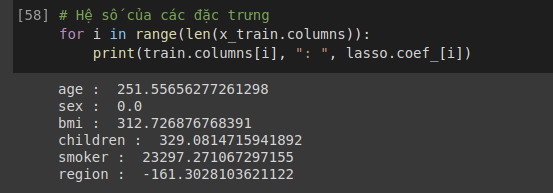
\includegraphics[width=0.75\textwidth]{images/lasso_reg/lasso_features_slope.png}
		\end{figure}
		\item Dự đoán
		\begin{itemize}
			\item Trên tập huấn luyện
			\begin{figure}[H]
				\centering
				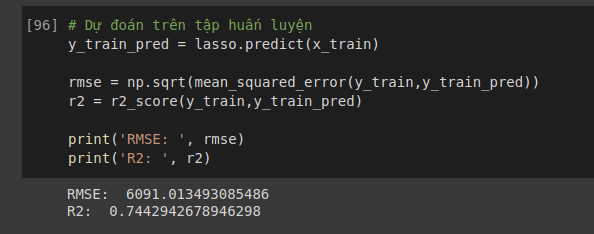
\includegraphics[width=0.75\textwidth]{images/lasso_reg/lasso_train_predict.png}
			\end{figure}
		Các đánh giá thực hiện kiểm tra mô hình trên tập huấn luyện, xem xét hai độ đo
		\begin{itemize}
			\item RMSE:  6091.013493085486, chỉ số này tương đối nhỏ
			\item R2:  0.7442942678946298, chỉ số này khá gần 1.0
		\end{itemize}
			\item Trên tập kiểm tra
			\begin{figure}[H]
				\centering
				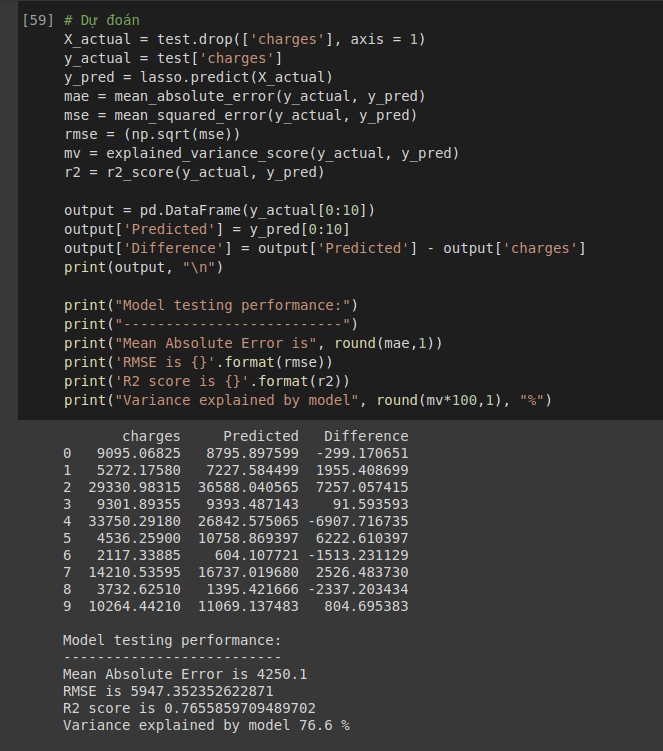
\includegraphics[width=0.75\textwidth]{images/lasso_reg/lasso_predict_test_data.png}
			\end{figure}
		Hiển thị bảng đối sánh kết quả thực và kết quả dự đoán, đánh giá thông qua các độ đo:
		\begin{itemize}
			\item Mean Absolute Error is 4250.1
			\item RMSE is 5947.352352622871
			\item R2 score is 0.7655859709489702
			\item Variance explained by model 76.56042\%
		\end{itemize}
		\end{itemize}
		\item Trực quan hóa
		\begin{figure}[H]
			\centering
			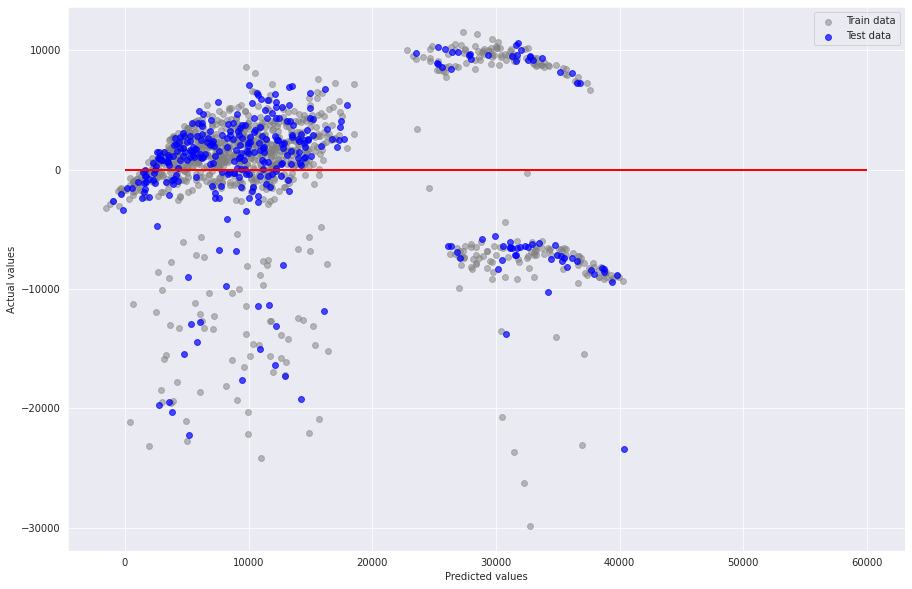
\includegraphics[width=0.75\textwidth]{images/lasso_reg/lass-reg_plot.png}
		\end{figure}
	\end{itemize}
	\textbf{Ưu điểm và nhược điểm của mô hình Hồi quy Lasso - Lasso Regression}
	\begin{itemize}
		\item Ưu điểm:
		\item Nhược điểm:
	\end{itemize}
	\subsubsection{Nhận xét}
	\begin{itemize}
		\item  tương tự với Ridge Regression, Lasso cũng tìm hệ dữ liệu với phương sai thấp nhất.
		\begin{itemize}
			\item $\text{Ridge tính toán predict} = \text{tổng bình phương phương sai thấp nhất với sai số là lambda} * \text{slope}^2$
			\item $\text{Lasso tính toán predict} = \text{tổng bình phương phương sai thấp nhất} + \lambda * \text{|slope|}$
		\end{itemize}
	\end{itemize}
	\subsection{5. Hồi quy rừng ngẫu nhiên - Random Forest Regressor}
	\subsubsection{Hồi quy rừng ngẫu nhiên cơ bản}
	\qquad Rừng ngẫu nhiên là một loại thuật toán Học Máy có giám sát dựa trên học tập theo nhóm (ensemble learning). Học theo nhóm (ensemble learning) là một kiểu học mà kết hợp nhiều loại thuật toán khác nhau hoặc cùng một thuật toán nhiều lần để tạo thành một mô hình dự đoán mạnh mẽ hơn. Thuật toán rừng ngẫu nhiên kết hợp nhiều thuật toán cùng loại, tức là nhiều cây quyết định, tạo ra một rừng cây, do đó có tên là "Rừng ngẫu nhiên". Thuật toán rừng ngẫu nhiên có thể được sử dụng cho cả nhiệm vụ hồi quy (regression) và phân loại (classification).
	
	Tóm tắt các bước của thuật toán Rừng ngẫu nhiên (Random Forest Algorithm)
	\begin{itemize}
		\item Chọn N bộ dữ liệu ngẫu nhiên từ tập dữ liệu.
		
		\item Xây dựng cây quyết định dựa trên N bộ dữ liệu này.
		
		\item Chọn số lượng cây người dùng muốn trong thuật toán của mình và lặp lại các bước 1 và 2.
		
		\item Trong trường hợp có vấn đề hồi quy, đối với một bản ghi mới, mỗi cây trong rừng dự đoán một giá trị cho Y (đầu ra). Giá trị cuối cùng có thể được tính bằng cách lấy giá trị trung bình của tất cả các giá trị được dự đoán bởi tất cả các cây trong rừng. Hoặc, trong trường hợp có vấn đề về phân loại, mỗi cây trong rừng dự đoán loại mà kỷ lục mới thuộc về. Cuối cùng, kỷ lục mới được gán cho hạng mục giành được đa số phiếu bầu. 
	\end{itemize}
	\begin{figure}[H]
		\centering
		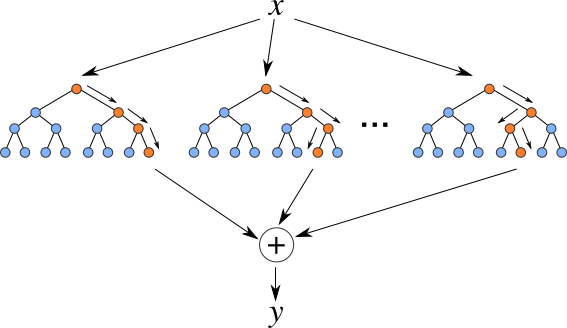
\includegraphics[width=0.75\textwidth]{images/random_forest_reg/model_overview.png}
	\end{figure}
	\begin{figure}[H]
		\centering
		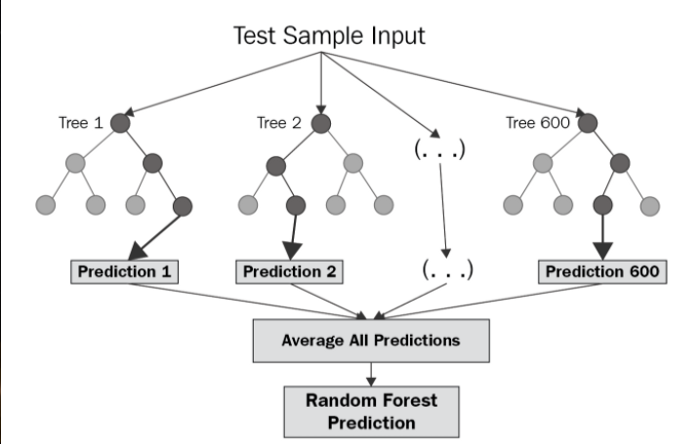
\includegraphics[width=0.75\textwidth]{images/random_forest_reg/random_forest_predict.png}
	\end{figure}
	\textbf{Ưu điểm - nhược điểm của thuật toán Rừng ngẫu nhiên}
	\begin{itemize}
		\item Ưu điểm:
		\begin{itemize}
			\item Thuật toán rừng ngẫu nhiên không sai lệch, vì có nhiều cây và mỗi cây được huấn luyện trên một tập dữ liệu con. Về cơ bản, thuật toán rừng ngẫu nhiên dựa vào sức mạnh của "đám đông"; do đó độ chệch tổng thể của thuật toán được giảm xuống.
			
			\item Thuật toán này rất ổn định. Ngay cả khi một điểm dữ liệu mới được đưa vào tập dữ liệu, thuật toán tổng thể không bị ảnh hưởng nhiều vì dữ liệu mới có thể ảnh hưởng đến một cây, nhưng rất khó để nó tác động đến tất cả các cây.
			
			\item Thuật toán rừng ngẫu nhiên hoạt động tốt khi dữ liệu có cả đặc trưng kiểu loại và kiểu số.
			
			\item Thuật toán rừng ngẫu nhiên cũng hoạt động tốt khi dữ liệu bị thiếu giá trị hoặc nó chưa được chia tỷ lệ tốt.
		\end{itemize}
		\item Nhược điểm:
		\begin{itemize}
			\item Độ phức tạp thuật toán, yêu cầu nhiều tài nguyên tính toán hơn, do số lượng lớn các cây quyết định được kết hợp với nhau.
			\item Do độ phức tạp thuật toán khá lớn nên thời gian huấn luyện mô hình cũng mất nhiều thời gian
		\end{itemize}
	\end{itemize}
	\subsubsection{Sklearn Hồi quy rừng ngẫu nhiên}
	Các bước thực hiện Hồi quy Lasso với thư viện Sklearn
	\begin{itemize}
		\item Chuẩn bị dữ liệu
		\begin{figure}[H]
			\centering
			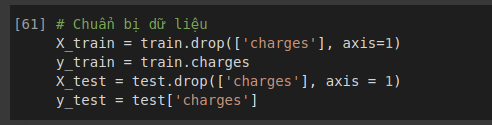
\includegraphics[width=0.75\textwidth]{images/random_forest_reg/random_forest_data_preparation.png}
		\end{figure}
		Tập dữ liệu huấn luyện, tập dữ liệu kiểm tra được đọc từ hai tập tin được cung cấp là train.csv và test.csv bằng Pandas, có dạng là data frame
		\item Khởi tạo mô hình và khớp dữ liệu trên tập huấn luyện
		\begin{figure}[H]
			\centering
			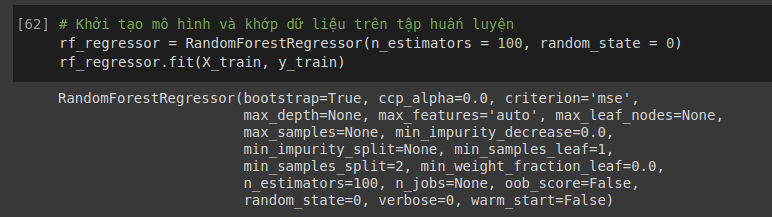
\includegraphics[width=0.75\textwidth]{images/random_forest_reg/random_forest_init_fit.png}
		\end{figure}
		\item Điểm số đóng góp của các đặc trưng
		Thể hiện mức độ quan trọng của đặc trưng của bộ dữ liệu. Theo những nhận định trong giai đoạn phân tích và trực quan hóa dữ liệu, đặc trưng tình trạng hút thuốc được nhóm nhận định là đặc trưng có ảnh hưởng khá lớn đối với chi phí cá nhân, và ở đây một lần nữa được kiểm chứng
		
		\begin{figure}[H]
			\centering
			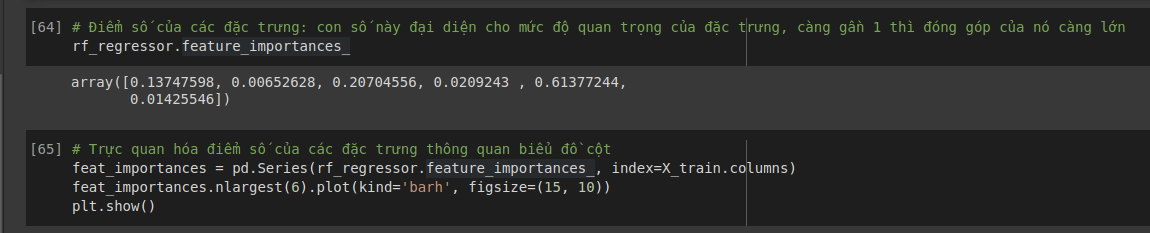
\includegraphics[width=0.75\textwidth]{images/random_forest_reg/random_forest_important_features.png}
		\end{figure}
		Nếu như ở trên, những thuật toán máy học khác cho thấy hệ số của đặc trưng này tương đối lớn khá nhiều so với các đặc trưng còn lại. Thông qua tính toán important features rate, ta dễ dàng trực quan hóa và thấy rõ ràng mức độ quan trọng của từng đặc trưng qua biểu đồ dưới đây
		\begin{figure}[H]
			\centering
			\includegraphics[width=0.75\textwidth]{images/random_forest_reg/random_forest_features_important_rate.png}
		\end{figure}
		\item Dự đoán
		\begin{itemize}
			\item Tập huấn luyện
			\begin{figure}[H]
				\centering
				\includegraphics[width=0.75\textwidth]{images/random_forest_reg/random_forest_train_predict.png}
			\end{figure}
		Các đánh giá thực hiện kiểm tra mô hình trên tập huấn luyện, xem xét hai độ đo
		\begin{itemize}
			\item RMSE:  1870.7046036122138
			\item R2:  0.9758803072907702
		\end{itemize}
			\item Tập test
			\begin{figure}[H]
				\centering
				\includegraphics[width=0.75\textwidth]{images/random_forest_reg/random_forest_predict_test_evaluation.png}
			\end{figure}
		Hiển thị bảng đối sánh kết quả thực và kết quả dự đoán, đánh giá thông qua các độ đo:
		\begin{itemize}
			\item Mean Absolute Error is 2601.5
			\item RMSE is 4798.365892312577
			\item R2 score is 0.8474110853586974
			\item Variance explained by model 84.80841\%
		\end{itemize}
		\end{itemize}
		\item Trực quan 
		\begin{figure}[H]
			\centering
			\includegraphics[width=0.75\textwidth]{images/random_forest_reg/random_forest_plot.png}
		\end{figure}
	\end{itemize}
	\subsubsection{Nhận xét}
	\begin{itemize}
		\item các bước thực hiện RFR
		\begin{itemize}
			\item Tạo ra bộ dữ liệu bootstrapped để 1 phần dữ liệu train. Tạo bộ cây quyết định bằng bộ dữ liệu bootstrapped tỉ lệ 1-1.
			\item Bộ dữ liệu trên được xem là random forest.
			\item Phần dữ liệu còn lại của bộ train được sử dụng để tính độ chính xác của rừng cây. Bằng cách cho những bộ dữ liệu đi qua từng bootstrap ( rừng bootstrap) ta có thể tính được tỉ lệ đúng sai của rừng cây đó.
			\item Sau khi tính được độ đúng sai của rừng. chúng ta quay lại bước 1 và tạo ra những rừng cây mới với cấu trúc khác.
			\item So sánh độ đúng sai của những rừng cây được tạo ra và chọn rừng cây phù hợp nhất.
		\end{itemize}
		\item Thuật toán cho kết quả khả quan trên tập huấn luyện và cả tập kiểm tra vối chỉ số $R^2$ cao, giải thích phương sai đạt 84.8\%, có RMSE tương đối thấp trên cả tập huấn luyện và tập kiểm tra		
	\end{itemize}
	\subsection{6. Hồi quy đa thức - Polynomial Regression}
	\subsubsection{Hồi quy đa thức cơ bản}
	\qquad Một mô hình được xem là tuyến tính nếu nó tuyến tính với những tham số
	\begin{align*}
		Y = \beta_0 + \beta_1X + \beta_2X^2 + \epsilon
	\end{align*}
	và 
	\begin{align*}
	Y = \beta_0 + \beta_1X_1 + \beta_2X_2 +  \beta_12X_1X_2 + \beta_{11}X_1^2 + \beta_{22}X_2^2 + \epsilon
	\end{align*}
	lần lượt là đa thức bậc một và bậc hai cũng được xem là môt hình tuyến tính (linear model)
	
	\subsubsection{Sklearn Hồi quy đa thức}
	Các bước thực hiện Hồi quy đa thức với thư viện Sklearn
	\begin{itemize}
		\item Chuẩn bị dữ liệu
		\begin{figure}[H]
			\centering
			\includegraphics[width=0.75\textwidth]{images/polynomial_reg/poly_data_preparation.png}
		\end{figure}
		\item Chọn bậc đa thức tối ưu
		\begin{figure}[H]
			\centering
			\includegraphics[width=0.75\textwidth]{images/polynomial_reg/poly_reg_choose_degree.png}
		\end{figure}
		\begin{figure}[H]
			\centering
			\includegraphics[width=0.75\textwidth]{images/polynomial_reg/poly_choose_degree.png}
		\end{figure}
		\item Khởi tạo mô hình và huấn luyện
		\begin{figure}[H]
			\centering
			\includegraphics[width=0.75\textwidth]{images/polynomial_reg/poly_init_fit.png}
		\end{figure}
		\item Dự đoán
		\begin{itemize}
			\item Trên tập huấn luyện
			\begin{figure}[H]
				\centering
				\includegraphics[width=0.75\textwidth]{images/polynomial_reg/poly_predict_train_set.png}
			\end{figure}
			\item Trên tập test
			\begin{figure}[H]
				\centering
				\includegraphics[width=0.75\textwidth]{images/polynomial_reg/poly_predict_test_evaluation.png}
			\end{figure}
		\end{itemize}
		\item Trực quan kết quả
		\begin{figure}[H]
			\centering
			\includegraphics[width=0.75\textwidth]{images/polynomial_reg/poly_reg_plot.png}
		\end{figure}
	\end{itemize}
	\subsubsection{Nhận xét}
	\begin{itemize}
		\item Polynomial Regression tiến bộ hơn so với Linear regression.
		\item Polynomial Regression thay đổi giá trị phụ thuộc theo từng data được train và tiến bộ dần với bộ dữ liệu lớn.
		\item Polynomial nhạy cảm với các outlier, tuy nhiên với bộ dữ liệu y tế trên, Polynomial không bị ảnh hưởng nhiều do được phát triển đủ tốt để thực hiện dự đoán với sai số thấp.
		\item Công thức chung Polynomial $\text{Predict} = \text{intercept} + \theta_1 \times (\text{slopeSex} * \text{dataSex} + \text{slopeBMI} \times \text{dataBMI} + ... ) + \theta_2 \times (\text{slopeSex} \times \text{dataSex} + \text{slopeBMI} \times \text{dataBMI} + ... ) + \theta_3 * (\text{slopeSex} \times \text{dataSex} + \text{slopeBMI} \times \text{dataBMI} + ... )$
	\end{itemize}
	\section{4. Các kết quả và nhận xét}
	
	\nocite{*}
	\bibliography{references}\newpage\cleardoublepage
	\bibliographystyle{plain}
	
\end{document}